\chapter{PV power plant with adapted EES}
\section{Design and simulation} \label{section PV system}
For this simulation a PV power plant was extended with an electrical energy storage (EES). This extended PV power plant was simulated in SAM's "Photovoltaic (detailed)" model with enabled battery storage option. Also for this simulation was the EPW weather file for Upington from Section~\ref{Location and weather data} used. For the PV simulation SAM uses the following input data:
\begin{itemize}
\item Latitude ($\,^{\circ}$)
\item Longitude ($\,^{\circ}$)
\item Elevation above sea level (\si{\metre})
\item GHI, DNI and DHI (\si{\watt\per\square\metre})
\item Dry bulb temperature (\si{\celsius})
\item Wind velocity (\si{\metre\per\second})
\end{itemize}
This section describes in detail the residual input data of the PV power plant with adapted battery storage. As before in the sections of simulated CSP technologies first the essential components of the system are defined. The financial parameters and the LCOE for this simulation was also here calculated separately and is documented in Appendix~\ref{ChapterLCOE} on Page \pageref{ChapterLCOE}.



As mentioned at the beginning of these Chapter this must be seen as theoretical simulation. Actually there are not that large electrical energy storage systems in form of battery storage available.



For this simulation the load was conected to the PV and Battery system as shown on Figure~\ref{PV_model_config}. The load shape was defined as before specified before in Chapter~\ref{Overall simulated configuration} and simulates the demand of the power grid. As it is shown there is also the actual power grid connected as additional component, but for this simulation just the power flows between PV, battery and load is in focus. As it is shown in the Figure, SAM actually just support the battery connection at the AC-bus via a power conversion system and is not able to simulate direct DC-connected batteries besides the PV-array before the PV-inverter. However in order to produce comparable results SAM was also used for the simulation of the PV power plant. As mentioned before this system contains out of the PV system with solar modules, solar and inverter and are described in the following section as well as the electrical energy storage.
\begin{figure}[htbp]  
\centering
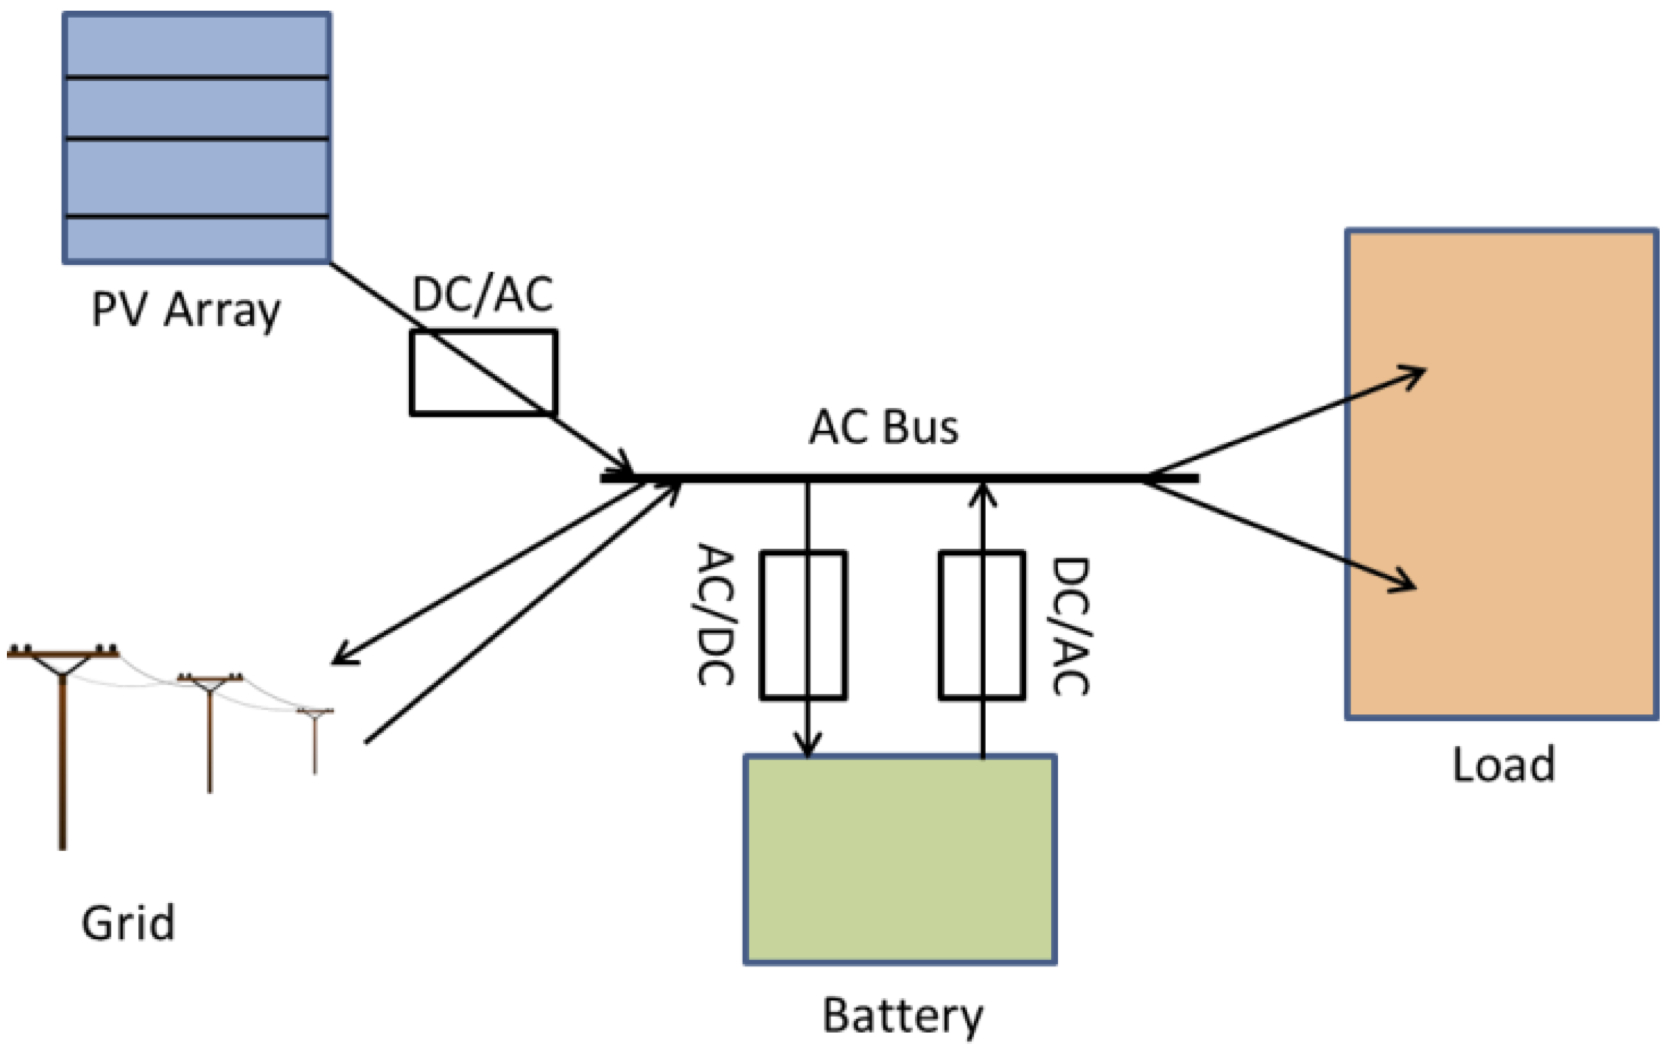
\includegraphics[width=0.55\linewidth]{FIG/PV_model_config}
\caption[Model of the configurated PV plus batterie scheme.]{Model of the configurated PV plus batterie scheme \cite{Diorio2015}.}\label{PV_model_config}
\end{figure}
\subsubsection{Simulated configurations}
The configurations of the PV system with adapted electrical energy storage has also the target to reach 90~\% of the scheduled production curve from Section~\ref{Overall simulated configuration}. To reach this target it is necessary to over scale the energy production of the PV system to produce enough power to covers the given load and load the storage during the day. This is quite similar to the solar multiple of the CSP system, but can not be put on a same level. Therefore this over scaling will be called "PV multiple" (PVM) and means the multiple of the PV inverter output. For example the system with a maximum inverter output of \SI{100}{\mega\wattel} is a PVM of 1 than has the PV system with a PVM of 2 a maximum inverter output of \SI{200}{\mega\wattel}. 
\begin{table}[htbp]  
  \centering
	\begin{tabular}{ p{4.0cm}  C{1.0cm} C{0.3cm} C{0.3cm} C{0.3cm} C{0.3cm} C{0.3cm}  | C{0.3cm} C{0.3cm} C{0.3cm} C{0.3cm} C{0.3cm} } 
	\hline	
\textbf{Item} & \textbf{Unit} & \multicolumn{10}{c}{\textbf{Value}} \\ \hline \hline
Maximum load supply & \si{\mega\wattel} & \multicolumn{10}{c}{100} \\ \hline
PV multiple & - & \multicolumn{5}{c}{1.0} & \multicolumn{5}{c}{1.8} \\
EES capacity & h & \multicolumn{5}{c}{-} & 4 & 5 & 6 & 7 & 8 \\ \hline 
PV multiple & - & \multicolumn{5}{c}{2.0} & \multicolumn{5}{c}{2.2} \\
EES capacity& h &  4 & 5 & 6 & 7 & 8 & 4 & 5 & 6 & 7 & 8 \\ \hline 
PV multiple & - & \multicolumn{5}{c}{2.4} & \multicolumn{5}{c}{2.6} \\
EES capacity & h & 4 & 5 & 6 & 7 & 8 & 4 & 5 & 6 & 7 & 8 \\ \hline 
\end{tabular}
\caption[Simulated configurations of the PV system with adapted EES.]{Simulated configurations of the PV system with adapted EES.}\label{tbl: PV_OverallConfig}
\end{table}
The simulated system load is maximum \SI{100}{\mega\wattel}, so this is also the maximum supply of the system. The PV system was simulated one time without storage and a maximum inverter output of \SI{100}{\mega\wattel} which is a PVM of 1. After that, the system was simulated in steps 0.2 of the PVM from 1.8 to 2.6. The adapted energy storage capacity was simulated from 4 to 8 hours in hourly steps. This storage capacity range is also defined for large-scale off-grid application in \cite{IEA2014c}. Table~\ref{tbl: PV_OverallConfig} summarizes the simulated configurations.
\subsubsection{PV system}
The simulated PV system is orientated at actual PV systems in SA. Therefore the currently under construction situated Mulilo Sonnedix Prieska PV Project in the Northern Cape will serve as a role model for the main components. In this \SI{75}{\mega\wattsdc}-project are poly crystalline \SI{305}{\wattsdc} modules of type BYD 305P6C-36 from BYD installed. The efficiency of the modules is about 15.72~\%. The full module specification is in Table~\ref{tbl: PVmodule}. The peak performance of the project is \SI{86.23}{\mega\wattsdc}. \cite{Morse2014}

\begin{table}[htbp]  
  \centering
	\begin{tabular}{  p{5.0cm}  C{5.0cm}  C{1.4cm} } 
	\hline	
\textbf{Item} & \textbf{Value} & \textbf{Unit} \\ \hline \hline
Manufacturer  & BYD COMPANY LIMITED & - \\ 
Model & BYD 305P6C-36 & - \\ 
Cell type &  poly-crystalline silicon & - \\ \hline
Maximum power & 304.99 & \si{\wattel} \\ 
Nominal efficiency & 15.72 & \si{\percent} \\ 
Maximum power voltage & 36.2 & \si{\voltsdc} \\ 
Maximum power current & 8.4 & \si{\ampsdc}  \\
Open circuit voltage & 45.5 & \si{\voltsdc}  \\ 
Short circuit current & 8.9 & \si{\ampsdc}  \\
Temperature efficiency & -0.41 & \si{\percent\celsius}\\
Module area & 1.94 & \si{\square\metre} \\ 
Number of cells & 72 & -\\
\hline
\end{tabular}
\caption[Module specification of BYD 305P6C-36.]{Module specification of BYD 305P6C-36 under STC: \SI{1000}{\watt\per\square\metre}, cell temperature \SI{25}{\celsius} \cite{NREL2015g}.}\label{tbl: PVmodule}
\end{table}


These for the simulation selected module type was already deposited in the module library in SAM. This large library is based on the database of Go Solar California for photovoltaic modules and inverters from the California Energy Commission \cite{NREL2015g}.

\begin{figure}[htbp]  
\centering
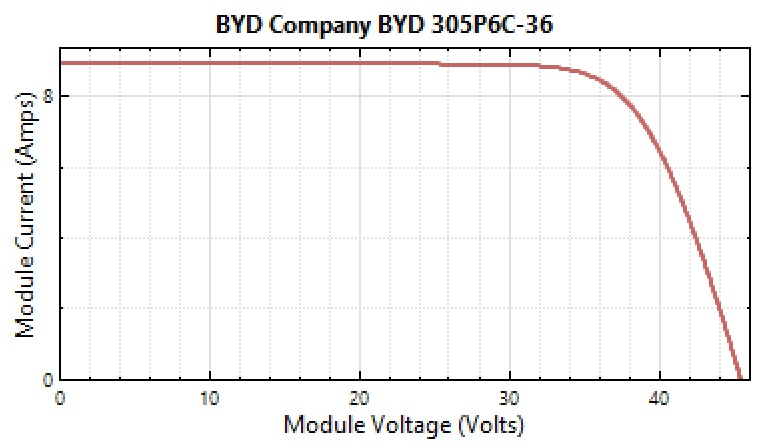
\includegraphics[width=0.70\linewidth]{FIG/PVModuleVA}
\caption[Current–voltage characteristic under STC of module BYD 305P6C-36.]{Current–voltage characteristic under STC of module BYD 305P6C-36 \cite{NREL2015g}.}\label{PVModuleVA}
\end{figure}


Figure~\ref{PVModuleVA} shows the module’s current–voltage characteristic with a short circuit voltage of \SI{8.9}{A} and an open circuit voltage of \SI{45.5}{V}.\newpage\noindent
The Mulilo Sonnedix Prieska PV Project install inverter from AEG. These specific AEG Protect PV.800 inverter is not available in the library of SAM, but a similar model with almost the same power rating was selected. Table~\ref{tbl: PVinverter} depicts the specifications of the for the simulation used Ingeteam inverter INGECON SUN 805TL U X420 Outdoor with \SI{805}{kW}\textsubscript{ac} power at an efficiency of 98.33~\%. The efficiency curve of the inverter can be seen in Figure~\ref{InverterEfficiencyCurve}. 

\begin{figure}[htbp]  
\centering
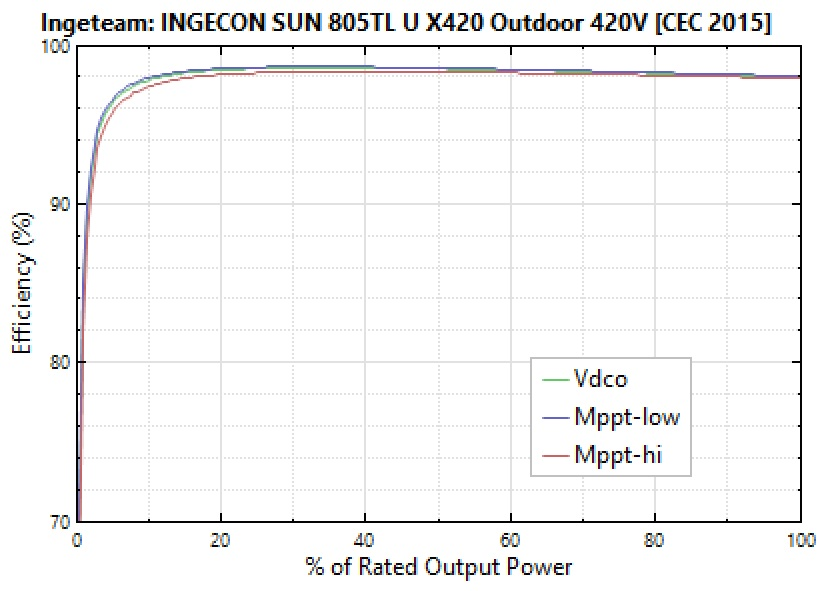
\includegraphics[width=0.75\linewidth]{FIG/InverterEfficiencyCurve}
\caption[Efficientcy characteristic of Ingecon Sun 805TL U X420 Outdoor.]{Efficientcy characteristic of Ingecon Sun 805TL U X420 Outdoor \cite{IngeteamINC.2015,NREL2015g}.}\label{InverterEfficiencyCurve}
\end{figure}
\begin{table}[htbp]  
  \centering
	\begin{tabular}{ p{6.0cm}  C{7.0cm}  C{1.5cm} } 
	\hline	
\textbf{Item} & \textbf{Value} & \textbf{Unit} \\ \hline \hline
Manufacturer  & Ingeteam Power Technology & - \\ 
Model & Ingecon Sun 805TL U X420 Outdoor & - \\ 
Type &  central inverter & - \\ \hline
\textbf{Input (dc)} &  &  \\ 
Maximum power & 821.39 & kW\textsubscript{dc} \\ 
Voltage range & 611-820 & V\textsubscript{dc} \\ 
Maximum voltage & 1~000 & V\textsubscript{dc} \\ 
Maximum current & 1~350 & A\textsubscript{dc} \\
Nominal voltage & 715.91 & V\textsubscript{dc} \\ \hline
\textbf{Output (ac)} &  &  \\ 
Maximum power & 805 & kW\textsubscript{ac} \\ 
Nominal voltage & 420 & V\textsubscript{ac} \\
Maximum current & 1.35 & A\textsubscript{ac} \\
Frequency & 50-60 & Hz \\
cos$\phi$ & 1 & -\\ \hline
Maximum efficiency & 98.33 & \\% 
European efficiency & 98.29 & \\% 
Power consumption in operation &1.25 & kW\textsubscript{dc} \\ 
Power consumption at night & 0.12 & kW\textsubscript{ac} \\ 
\hline
\end{tabular}
\caption[Inverter specifications of Ingecon Sun 805TL U X420 Outdoor.]{Inverter specifications of Ingecon Sun 805TL U X420 Outdoor \cite{IngeteamINC.2015,NREL2015g}.}\label{tbl: PVinverter}
\end{table}
\newpage\noindent
As mentioned before the PV system was design under similar condition that the Mulilo Sonnedix Prieska PV Project. There a dc/ac ratio of 1.15 is used \cite{Morse2014}. This power ratio compares the photovoltaic array power to the inverter capacity \cite{Woodcock2013}. For the simulated PV system the same ratio was assumed. So at 100 MW\textsubscript{ac} inverter output, a total module capacity of 115 MW\textsubscript{dc} is needed. From the discussed parameter and the PVM SAM calculates the resulting number of modules and inverters as well as other parameters on its own. These PV system parameter are summarized in Table~\ref{tbl: PVsystemdesign}.

\begin{table}[!b]  
  \centering
	\begin{tabular}{ p{4.5cm} C{1.0cm} C{1.2cm} C{1.2cm} C{1.2cm} C{1.2cm} C{1.2cm} C{1.2cm} } 
	\hline	
\textbf{Item} & \textbf{Unit} & \multicolumn{6}{c}{\textbf{Value}} \\ \hline \hline
Module azimuth & $\,^{\circ}$ &\multicolumn{6}{c}{0 (north)}\\
Module tilt & $\,^{\circ}$ & \multicolumn{6}{c}{28.4}\\
Modules per string& - & \multicolumn{6}{c}{21}\\
String open circuit voltage& V\textsubscript{oc} & \multicolumn{6}{c}{955.3}\\
String max. power rated voltage& V\textsubscript{mp} & \multicolumn{6}{c}{759.8}\\
Maximum dc-voltage& V\textsubscript{dc} & \multicolumn{6}{c}{1~000}\\
Aspired dc/ac-ratio & - &\multicolumn{6}{c}{1.15}\\
\hline
\textbf{PV multiple} & - & \textbf{1.0} & \textbf{1.8} & \textbf{2.0} & \textbf{2.2} & \textbf{2.4} & \textbf{2.6}\\ \hline 
Total inverter capacity & MW\textsubscript{ac} & 99.8 & 180.3 &199.6 & 219.8 & 239.9 & 260.0 \\
Total module capacity & MW\textsubscript{dc} & 115.0 & 207.0 & 230.0 &253.0 & 276.0 & 299.0 \\
Strings in parallel & - & 17~954 & 32~318 & 35~909 & 39~500 & 43~091 & 46~682 \\
Number of modules & - & 377~034 & 678~678& 754~089 & 829~500 & 904~911 & 980~322 \\
Number of inverter  & - & 124 & 224 & 248 & 273 & 298 & 323 \\
Total module area & ha & 73.1 & 131.7 & 146.3 & 160.9 & 175.6 & 190.1 \\
Total land area & ha & 244 & 439 & 488 & 536 & 585 & 634 \\
\hline
\end{tabular}
\caption[PV system design parameter.]{PV system design parameter.}\label{tbl: PVsystemdesign}
\end{table}

For the orientation of the simulated PV-modules the latitude of Upington was used as tilt angle (28.4$\,^{\circ}$) and the azimuth is 0$\,^{\circ}$, so directly facing north. The self-shading model was selected, without external shading parameter. Therefore 2 modules along the side of row and 10 along the bottom of row was selected. Therefrom a shading loss of 0.545~\% on the solar radiation incident on the subarray. Further assumed losses are soiling, mismatch, diodes and connections and wiring losses. The assumed soiling losses reduce the solar radiation incident on the subarray of about 5~\%. The assumed mismatch loss of about 2~\% is related to slight differences in performance of individual modules in the array. Voltage drops across blocking diodes and electrical connections leads to a assumed diodes and connections loss of 0.5~\%. There are also assumed resistive losses of 2~\% in wiring on the dc-side and 1~\% wiring loss between the inverter and the grid connection point on the ac-side of the system. All PV system loss parameter coming from a IEEE photovoltaics specialists conference paper about performance parameters for grid-connected PV systems \cite{Marion2005}.
\subsubsection{Electrical energy storage (EES)}
The electrical energy storage is adapted though the system as it is shown in Figure~\ref{PV_model_config} on Page~\pageref{PV_model_config}. The EES basically consists out of two parts - the power conversions system (PCS) and the storage unit - as it is shown in Figure~\ref{TCC_EES} on Page~\pageref{TCC_EES}. For the simulation in SAM the PCS was simplified to the conversion efficiency. The AC to DC conversion efficiency was assumed with 99~\% as well as the DC to AC efficiency. Nevertheless for the LCOE calculation it is still relevant to define the performance of the PCS. As it is shown in Table~\ref{tbl: PVsystemdesign} the inverter capacity range is between 240 and \SI{320}{MW}\textsubscript{ac} for the simulation cases with adapted storage. The maximum scheduled load from Section~\ref{Overall simulated configuration} is \SI{100}{MW}. So depending from the PV inverter capacity the PCS capacity needs to variate as well to collect the  PV-overproduction. For the calculation of the LCOE it was assumed that the PCS needs to collects the inverter capacity minus the \SI{100}{MW} daily base load.



As mentioned before the storage unit consists out of a Li-Ion battery, more precisely a using a Nickel Cobalt Aluminum ($LiNiCoAlO_2$  or NCA) cathode. This battery excels through a less expensive cathode material with improved safety characteristics and high specific energy \cite{NREL2015a}. The voltage characteristics of these battery for the simulation are shown in Figure~\ref{EES_VoltageDischarge}. The NCA battery is inter alia installed in the Tesla Model S and X \cite{Nykvist2015} which uses currently Panasonic cells and will also be installed in Teslas Power Wall system \cite{Shahan2015}. The performance and lifetime of the NCA batteries depending on how they are used. Tesla names the lifetime of 5~000 cycles without mentioning the assumed depth of discharge (DOD) \cite{Shahan2015}.

\begin{figure}[!htbp]  
\centering
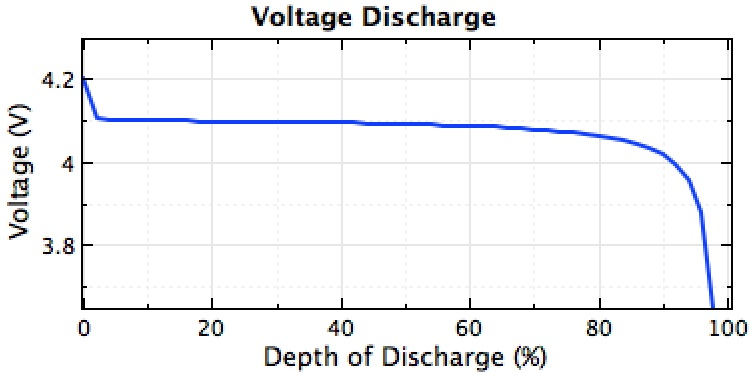
\includegraphics[width=0.6\linewidth]{FIG/EES_VoltageDischarge}
\caption[Voltage proparties of NCA Li-Ion battery.]{Voltage proparties of NCA Li-Ion battery..}\label{EES_VoltageDischarge}
\end{figure}



The DOD is the amount of capacity in the battery that is usable by the system. For electric vehicles (EV) the DOD is set between 80-95~\% at the "top" end of the battery and 10-20~\% at the "bottom" end \cite{Warner2014}. The state of charge (SOC) is an expression of the present battery capacity as a percentage of maximum capacity and is the inverse of the DOD. It must be noted, that the nominal capacity of a battery is not the effective usable capacity of a battery and depends on the DOD. Also the DOD effects the cycle life of the batteries. The higher the DOD, the lower the cycle life. In other words, the lower the SOC, the longer the cycle life. \cite{MitElectricVehilceTeam2008}



SAM visualizes the decreasing capacity of the battery over the number of cycles with capacity fades as it is shown in Figure~\ref{CapacityFade} for the NCA. The figure shows the characteristic for 20~\% and 80~\% DOD. As mentioned above the graph shows the higher decreasing of the effective capacity at higher DOD. The performance data behind this graph is coming from \cite{Dahn2011} and correspond with other tests \cite{Read2009}.
\begin{figure}[bhtp]  
\centering
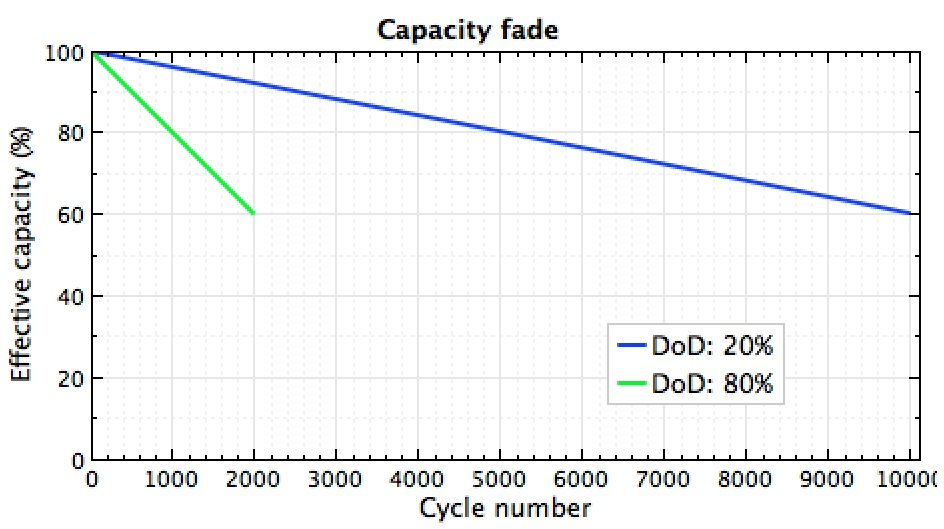
\includegraphics[width=0.75\linewidth]{FIG/CapacityFade}
\caption[Capacity fade of Nickel Cobalt Aluminum Lithium-Ion battery.]{Capacity fade of Nickel Cobalt Aluminum Lithium-Ion battery.}\label{CapacityFade}
\end{figure}

It must be noted, that the cycle lifetime is not only affected by the DOD but also by other conditions such as temperature and humidity \cite{MitElectricVehilceTeam2008}. SAM designs the cycle lifetime for the batteries at a constant room temperature of 20\si{\celsius} therefore the storage room needs to be conditioned. Also the charging and discharging of the battery results losses in form of heat which needs to get led away. The cooling demand of the EES system is not included in the simulation, but must be actually significant. \cite{Diorio2015} 



The system was designed for a lifetime of 25 years. Therefore also the EES is designed for this period. For the simulation a amount of 365 cycles per year was assumed. So the NCA was designed for 9~125 cycles whiteout using a battery bank replacement. SAM also can analyses the cycle lifetime of the batteries. This analyses showed that the NCA battery reaches this cycle lifetime with a DOD of 50~\%. But under this conditions the effective capacity of the battery is nearly 0~\% after 25 years. As it is shown in Figure~\ref{CapacityFade} the effective capacity of the NCA battery decreases almost lineal with the cycle number. There are two opportunities to reduce the loss to the effective capacity increasing over the lifetime of the system. First is a battery bank replacement after a specified schedule or loss of effective capacity to a specified amount and second is to use a lower DOD which leads also to a lower effective usable capacity of the battery, so a higher nominal capacity of the battery would be necessary.



Further is to note that Li-Ion batteries has a expiry period \cite{Jossen2006}. Tesla gives a warranty of 10 years of the batteries \cite{Shahan2015} so it can be expected, that the expiry period is close to these warranty. So also for the simulation an battery bank replacement is indispensable.



The for a long lifetime an average SOC of 30-70~\% is recommended for Li-Ion batteries \cite{Jossen2006}. Consequently the SOC was set to a maximum of 30~\% and a minimum of 70~\% for the simulation. So a total DOD of 40~\% which signified 40~\% of the nominal battery capacity was assumed as usable. In order to have high storage availability over the total system lifetime it was assumed that the battery bank will replaced at a effective capacity loss of 20~\%. This is also advised for EES in electronic consumer devices \cite{Spotnitz2003}. Resulting from this assumptions the cycle lifetime of the cells in the battery bank is 2~500 cycles. Therefore the battery bank needs to be replaced after 6-\SI{7}{years}. So the battery bank needs to be replaced three times in the total lifetime of the system. 



Table~\ref{tbl: EESsystemdesign} summarizes results of the discussed parameter for the simulation. The adapted voltage level for this large-scale EES application from \SI{820}{V}\textsubscript{dc}\ per string is coming from \cite{Leuthold2014}. The remaining values results from the above discussed parameter or are adapted from the SAM library \cite{Diorio2015}. 
\begin{table}[!htbp]  
  \centering
	\begin{tabular}{ p{5.0cm} C{1.0cm} C{1.2cm} C{1.2cm} C{1.2cm} C{1.2cm} C{1.2cm} } 
	\hline	
\textbf{Item} & \textbf{Unit} & \multicolumn{5}{c}{\textbf{Value}} \\ \hline \hline
Chemistry & - & \multicolumn{5}{c}{Lithium ion: nickel cobalt aluminum oxide} \\
Cell nominal voltage & V\textsubscript{dc} &\multicolumn{5}{c}{3.6}\\
Internal resistance & Ohm &\multicolumn{5}{c}{0.1}\\
Fully charged cell voltage & V\textsubscript{dc} &\multicolumn{5}{c}{4.2}\\
Exponential zone cell voltage & V\textsubscript{dc} &\multicolumn{5}{c}{4.1}\\
Nominal zone cell voltage & V\textsubscript{dc} &\multicolumn{5}{c}{3.6}\\
Nominal bank voltage & V\textsubscript{dc} &\multicolumn{5}{c}{820}\\
Cells in in series& - &\multicolumn{5}{c}{228}\\
Cell capacity & Ah &\multicolumn{5}{c}{55}\\
C-rate of discharge curve & - &\multicolumn{5}{c}{0.2}\\
Maximum C-rate charge & per/h &\multicolumn{5}{c}{1}\\
Maximum C-rate discharge & per/h &\multicolumn{5}{c}{1}\\
Total DOD& \% &\multicolumn{5}{c}{20}\\
\hline
\textbf{Storage capacity at \SI{100}{MW} output} & \textbf{h} & \textbf{4} & \textbf{5} & \textbf{6} & \textbf{7} & \textbf{8} \\ \hline 
Effective capacity & MWh & 400 & 500 & 600 & 700 & 800 \\
Nominal capacity & MWh & 1~000 & 1~250 & 1~500 & 1~750 & 2~000\\
Cells & $\times 10^6$ & 5.1 & 6.3 & 7.6 & 8.8 & 10.1\\
\hline
\end{tabular}
\caption[EES system design parameter.]{EES system design parameter.}\label{tbl: EESsystemdesign}
\end{table}
\pagebreak
\subsubsection{Financial parameter}
The financial parameter for the LCOE calculation are composed in Table~\ref{tbl: PVFinance}. As mentioned before was the LCOE calculation for this simulation made separately in Microfoft Excel using a simplified method which is documented in Appendix~\ref{ChapterLCOE} on Page \pageref{ChapterLCOE}. As for the other systems is the PV power plant designed for a lifetime of \SI{25}{years}. 

The specific large-scale PV system costs in South Africa  amount to \SI{1.285}{USD/W}\textsubscript{p} (\SI{14.5}{ZAR/W}\textsubscript{p} using \SI{11.286}{USD/ZAR} average in 2014 \cite{IRS2015}) which leads from an in 2014 actually built PV system \cite{Terblanche2015}. These specific costs are close to utility-scale PV systems in Europe with specific investments of \SI{1}{EUR/W}\textsubscript{p} \cite{FraunhoferISE2013}, corresponding to \SI{1.33}{USD/W}\textsubscript{p} (using the average exchange rate in 2014 of \SI{1.33}{USD/EUR}  \cite{StatistaGmbH2015}).

The LCOE was calculated with different interest rates and O\&M costs for the PV power plant and the EES system. The real interest rate for the PV power plant was amused with 2.8~\% \cite{FraunhoferISE2013} and the annual O\&M costs are 1~\%  of the PV investment costs \cite{IEA2014a}. A degradation of 1~\% per year of the annual energy output was assumed for the ageing phenomena of the PV cells \cite{Tidball2010}.

The storage costs are calculates from three  parts. The costs for the PCS, the battery bank and the replacement costs of the battery bank during the lifetime of the system.

The costs of the PCS of \SI{615}{USD/kW} (\SI{463}{EUR/kW} using the average exchange rate in 2014 of 1.33 USD/EUR \cite{StatistaGmbH2015}) was taken over from a study toward comparative life cycle cost analysis of EES \cite{Zakeri2015}. This is the average value of  a wide cost range (250-600€/kW) of PCS for Li-Ion EES systems.

For the storage part of the EES a highly optimistic value of \SI{300}{USD/kWh} was assumed from \cite{Nykvist2015}. The average storage part cost for Li-Ion EES in other studies is \SI{914}{USD/kWh} \cite{Zakeri2015}.

For the replacement costs of the an other highly optimistic value of \SI{150}{USD/kWh} was assumed. The cost for the replacement of the storage in \cite{Zakeri2015} are approximately the half of the storage costs. This costs was also assumed with a look to Figure~\ref{CostofLi-ion} on Page~\pageref{CostofLi-ion}.

The assumed EES battery bank replacements during the lifetime was described in this Chapter already.

The annual O\&M costs of \SI{9.18}{USD/kW} was also a adaption from \cite{Zakeri2015} as well as the real interest rate of 8.0~\%.

As before for the other solar power plants also for the PV system was land purchase costs of 3~000USD/ha \cite{Cassell2012} assumed.
\pagebreak
\begin{table}[!h]  
  \centering
	\begin{tabular}{  p{5.4cm} C{1.5cm} C{1.5cm}  C{1.7cm}  C{4.0cm} } 
	\hline	
\textbf{Item} & \textbf{Symbol}& \textbf{Value} & \textbf{Unit} & \textbf{Source}\\ \hline \hline
Lifetime &$n$ & 25 & years & \cite{FraunhoferISE2013} \\ \hline
Solar modules & $c_{sm}$&0.481 & USD/W\textsubscript{p} & \cite{Terblanche2015}\\ 
Structural &$c_{st}$ &0.138 & USD/W\textsubscript{p} & \cite{Terblanche2015} \\ 
Electrical parts &$c_{ep}$ &0.116 & USD/W\textsubscript{p} & \cite{Terblanche2015} \\ 
Inverters&$c_{inv}$ &0.117 & USD/W\textsubscript{p} & \cite{Terblanche2015} \\ 
Engineering and labour costs & $c_{elc}$ & 0.242 & USD/W\textsubscript{p} & \cite{Terblanche2015} \\ 
Security and infrastructure & $c_{si}$& 0.091 & USD/W\textsubscript{p} & \cite{Terblanche2015} \\ 
Transport and logistics & $c_{tl}$& 0.067 & USD/W\textsubscript{p} & \cite{Terblanche2015}\\ 
Sub-Station & $c_{ss}$ & 0.071 & USD/W\textsubscript{p} &\cite{Terblanche2015} \\ \hline
Total PV system costs & $c_{PV}$ & 1.285 &  USD/W\textsubscript{p} &\cite{Terblanche2015} \\ 
Annual degradation factor &$f_{degrad}$ & 1 & \% & \cite{Tidball2010}\\ 
Annual PV O\&M costs factor &$f_{O\&M,PV}$ & 1 & \% & \cite{IEA2014a}\\
Interest rate of PV & $i_{PV}$& 2.8 & \% & \cite{FraunhoferISE2013} \\ 
Annual insurance costs & $f_{ins,PV}$ & 0.5 & \% & \cite{InternationalFinanceCorporation2015}\\ \hline
EES PCS costs & $c_{EES,PCS}$ & 615 & USD/kW & \cite{Zakeri2015} \\ 
EES battery bank costs & $c_{EES,BBC}$ &300 & USD/kWh & \cite{Nykvist2015} \\ 
EES battery bank replacement costs & $c_{EES,BBRC}$ & 150 & USD/kWh & \cite{Zakeri2015} \\ 
Assumed EES battery bank replacements during lifetime & $n_{BBR}$ & 3 & - & - \\ 
Annual EES O\&M costs & $c_{O\&M,EES}$ & 9.18 & USD/kW & \cite{Zakeri2015}\\
Interest rate of EES & $i_{EES}$& 8.0 & \% & \cite{Zakeri2015} \\
Annual insurance costs& $f_{ins,EES}$ & 0.5 & \% & \cite{Cutter2014}\\ \hline
Land purchase &$c_{LP}$ & 3~000.00 & USD/ha & \cite{Cassell2012} \\ 
\hline
\end{tabular}
\caption[Finacial input parameter for PV-simulation in SAM.]{Finacial input parameter for PV-simulation in SAM.}\label{tbl: PVFinance}
\end{table}
\pagebreak
\section{Simulation results of PV power plant}
In this section the results of the simulated PV system and there belonging LCOE results are described and analyzed. First the PV system without EES and then the results of the PV system with adapted EES. The goal of these Section is to find the suitable PV power plant design configuration to reach a covering of 90~\% of the prescribed load which having the lowest belonging LCOE result.
\subsubsection{PV power plant without storage}
As it was described before at the beginning of Section~\ref{section PV system}, the PV system was also simulated without using an EES system. These PV system was designed for a maximum power output of \SI{99.8}{MW}\textsubscript{ac} and \SI{115.0}{MW}\textsubscript{dc} as it is defined in Table~\ref{tbl: PVsystemdesign}. It must be noted, that the following results are simulated for the first year of the PV system so for the performance results contains no degradation which is to be expected during the full lifetime. For the LCOE calculation a degradation factor was assumed as it was described in the previous section. 

Figure \ref{PVwithoutEESanual} visualizes the resulting annually load covering behavior. It can be seen, that the system can't cover the prescribed load at all. As it is usually for a solar powered system without storage the energy production standstill during the night time. The here shown annual average PV system power output covers about 32.9~\% of the prescribed load in the first year of the system. So the simulated PV system had a annual energy production during the first year of about \SI{233.69}{GWh}.

\begin{figure}[htbp]  
\centering
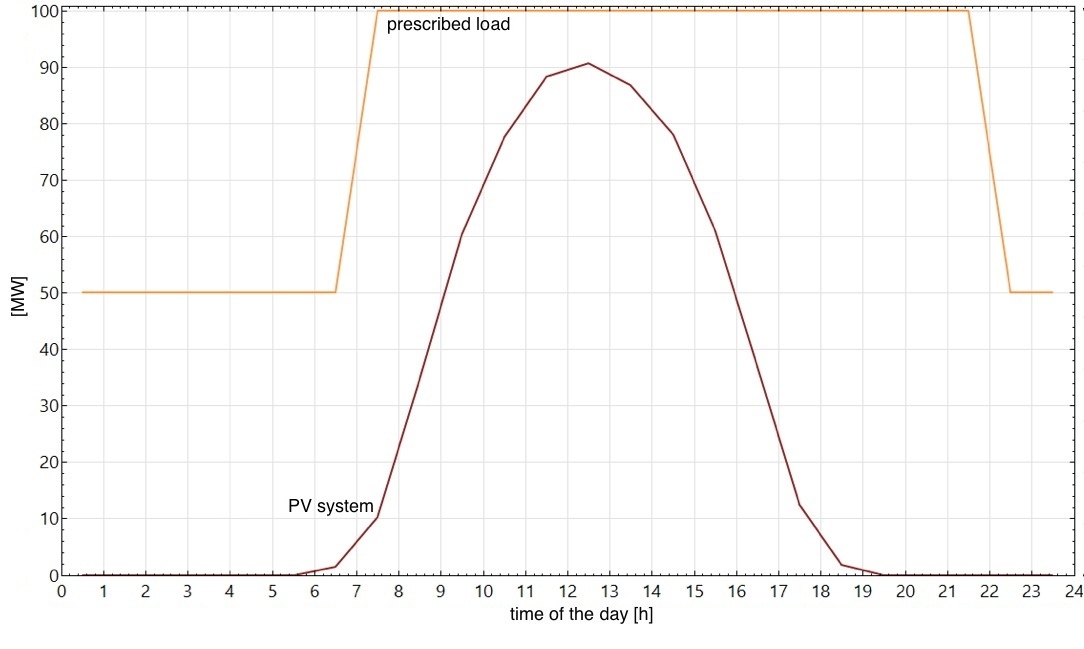
\includegraphics[width=0.8\linewidth]{FIG/PVwithoutEESanual}
\caption[Annual average profile of the simulated PV power plant without EES.]{Annual average profile of the simulated PV power plant without EES.}\label{PVwithoutEESanual}
\end{figure}
The simulation results of the energy output behavior in Figure~\ref{PVwithoutEES} shows that there is a small differences of the daily peak system power output between winter and summer time even though the GHI peak during the summer time is about twice that high then the winter peak. This leads from the irradiation angle of the sunlight and the fixed module tilt angle. However, the shorter sunshine duration reduces the daily energy output anyways. Especially appreciable is the situation at the noon of the 27. December. There the PV field produces more than the inverter can process because they reached there max output power of \SI{99.8}{\mega\watt}\textsubscript{ac}. At this day the PV system produces \SI{767}{\mega\watt\hour}, comparing this to the energy production at the 27. June (\SI{548}{\mega\watt\hour}) the difference in energy production between a summer and a winter day is just about \SI{29}{\percent}.

\begin{figure}[!htbp]
        \centering                
        \begin{subfigure}[b]{0.5\textwidth}
                \centering
                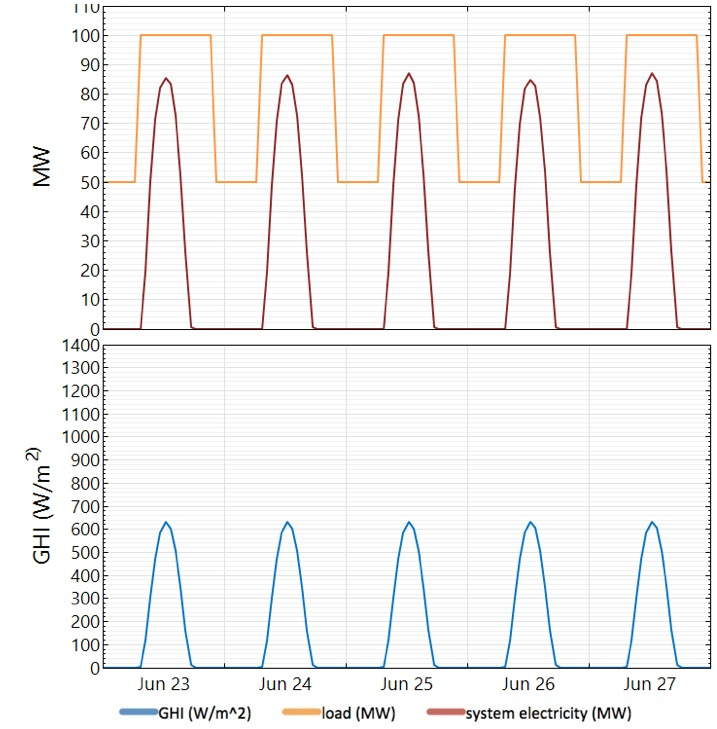
\includegraphics[width=1\textwidth]{FIG/PVwithoutEESwinter}
                \caption{Power output behavior short after winter solstice (23. to 27. June).}\label{PVwithoutEESwinter}
        \end{subfigure}%
        ~
        \begin{subfigure}[b]{0.5\textwidth}
                \centering
                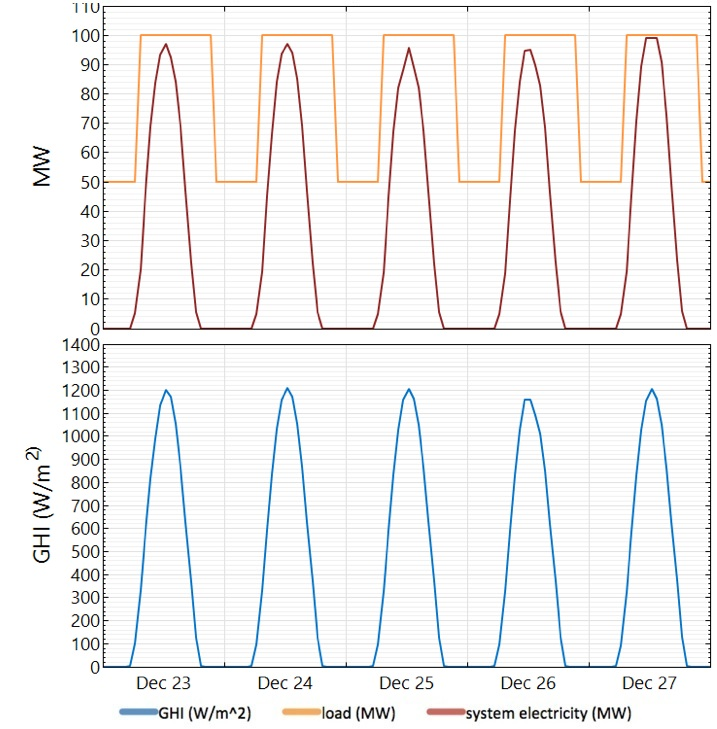
\includegraphics[width=1\textwidth]{FIG/PVwithoutEESsummer}
                \caption{Power output behavior short after summer solstice (23. to 27. December).}\label{PVwithoutEESsummer}
        \end{subfigure}
        \caption[Power output behavior of PV system.]{Power output behavior of PV system.}\label{PVwithoutEES}
\end{figure}
The LCOE was calculated taking into account of 1~\% annual degradation of the PV modules and under use of the remaining values from Table~\ref{tbl: PVFinance}. The LCOE was calculated using a the in Appendix~\ref{ChapterLCOE} documented method and results \SI{50.81}{USD/MWh}. Table~\ref{tbl: PVwithoutEESresult} summarizes the results of the PV system without adapted EES.
\begin{table}[htbp]  
  \centering
	\begin{tabular}{  p{3.0cm}  C{3.0cm}  C{3.0cm} } 
	\hline	
\textbf{Item} & \textbf{Value} & \textbf{Unit} \\ \hline \hline
First year energy & 233.69 & GWh \\ 
Load covering &  32.9 & \% \\ 
LCOE result & 50.81 & USD/MWh \\
\hline
\end{tabular}
\caption[Summary of the results of the simulated PV system without EES.]{Summary of the results of the simulated PV system without EES.}\label{tbl: PVwithoutEESresult}
\end{table}
\pagebreak
\subsubsection{Load curve covering}
The PV system was also simulated with the adapted EES system as it was described before in Section~\ref{section PV system}. In order to find a suitable size of the PV system and for the adapted EES, there was 25 different configurations simulated as they are described in Table~\ref{tbl: PV_OverallConfig}. The lowest defined configuration was simulated using a PVM of 2.0 and a \SI{4}{h} of EES. The highest simulation configuration was defined with a PVM of 2.8 and a EES capacity for \SI{8}{h} at \SI{100}{MW} output. In the following the simulation results of these configurations are delineated  representative for the remaining 23 configurations in between. 

The simulation results are based on the first year energy output of the designed PV power plants and don't includes degradation of the PV system or the adapted EES system. 

The result of the simulation for the both selected configurations are present in the annual average load profile in Figure~\ref{PV_annual_profil}. The simulation result shows that the highest configuration can cover the load almost completely during the simulated first year and just has appreciable shortfalls of covering in the morning hours. Considering the the load curve behavior from \SI{10}{am} to \SI{4}{pm} it can be noticed, that the predicted load is covered over the whole year in that time span. Compared to that covers the lowest PV power plant configuration much less of the predicted load curve. The  annual average load profile shows that during the night the system coming to standstill from 12 pm to 5 am over the full year. Nevertheless, the PV power plant can cover the prescribed load completely during the midday at any time of the year. The remaining  annual average load profile simulation results can be found in Appendix~\ref{all_load_profile}.

\begin{figure}[htbp]  
\centering
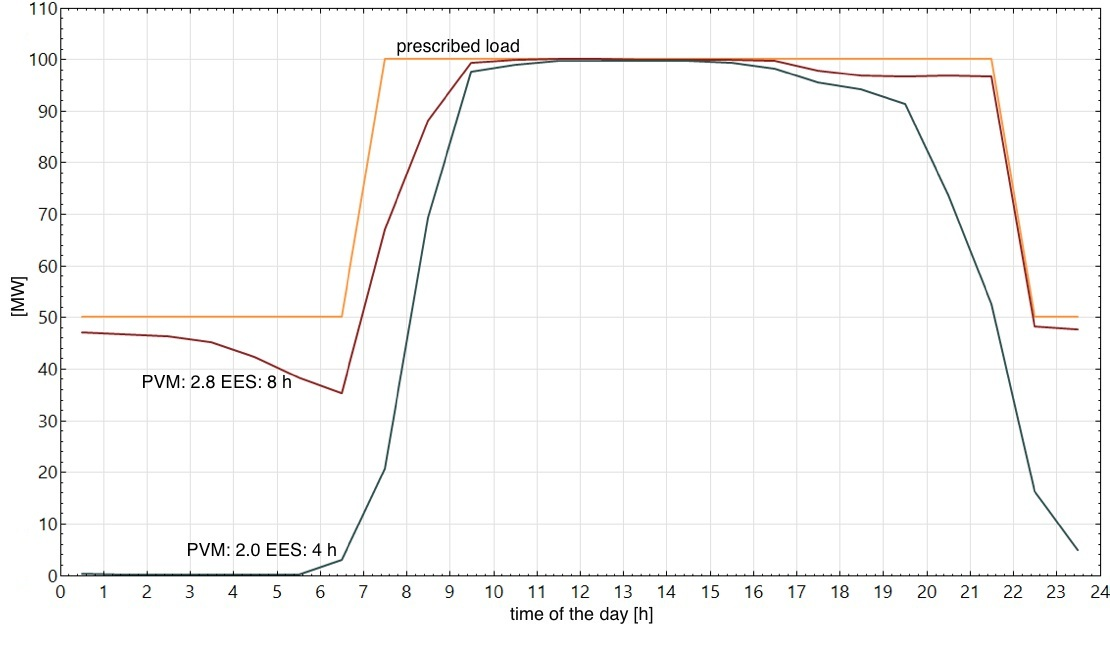
\includegraphics[width=0.8\linewidth]{FIG/PV_annual_profil}
\caption[Annual average load profile of selected PV power plant configurations.]{Annual average load profile of selected PV power plant configurations.}\label{PV_annual_profil}
\end{figure}
The covering of the prescribed load during the day results mainly from the PV system, which also loads with there surplus power production the EES. During the night the EES taken over the covering of the load till it reaches the fixed bottom limit of the SOC. If the EES is fully loaded and the PV system is still producing more electricity than the prescribed load needs the surplus power is not going in to the load curve covering calculation as well as into the LCOE calculation as it was defined in Section~\ref{Overall simulated configuration}. 

\begin{figure}[!bhtp]  
\centering
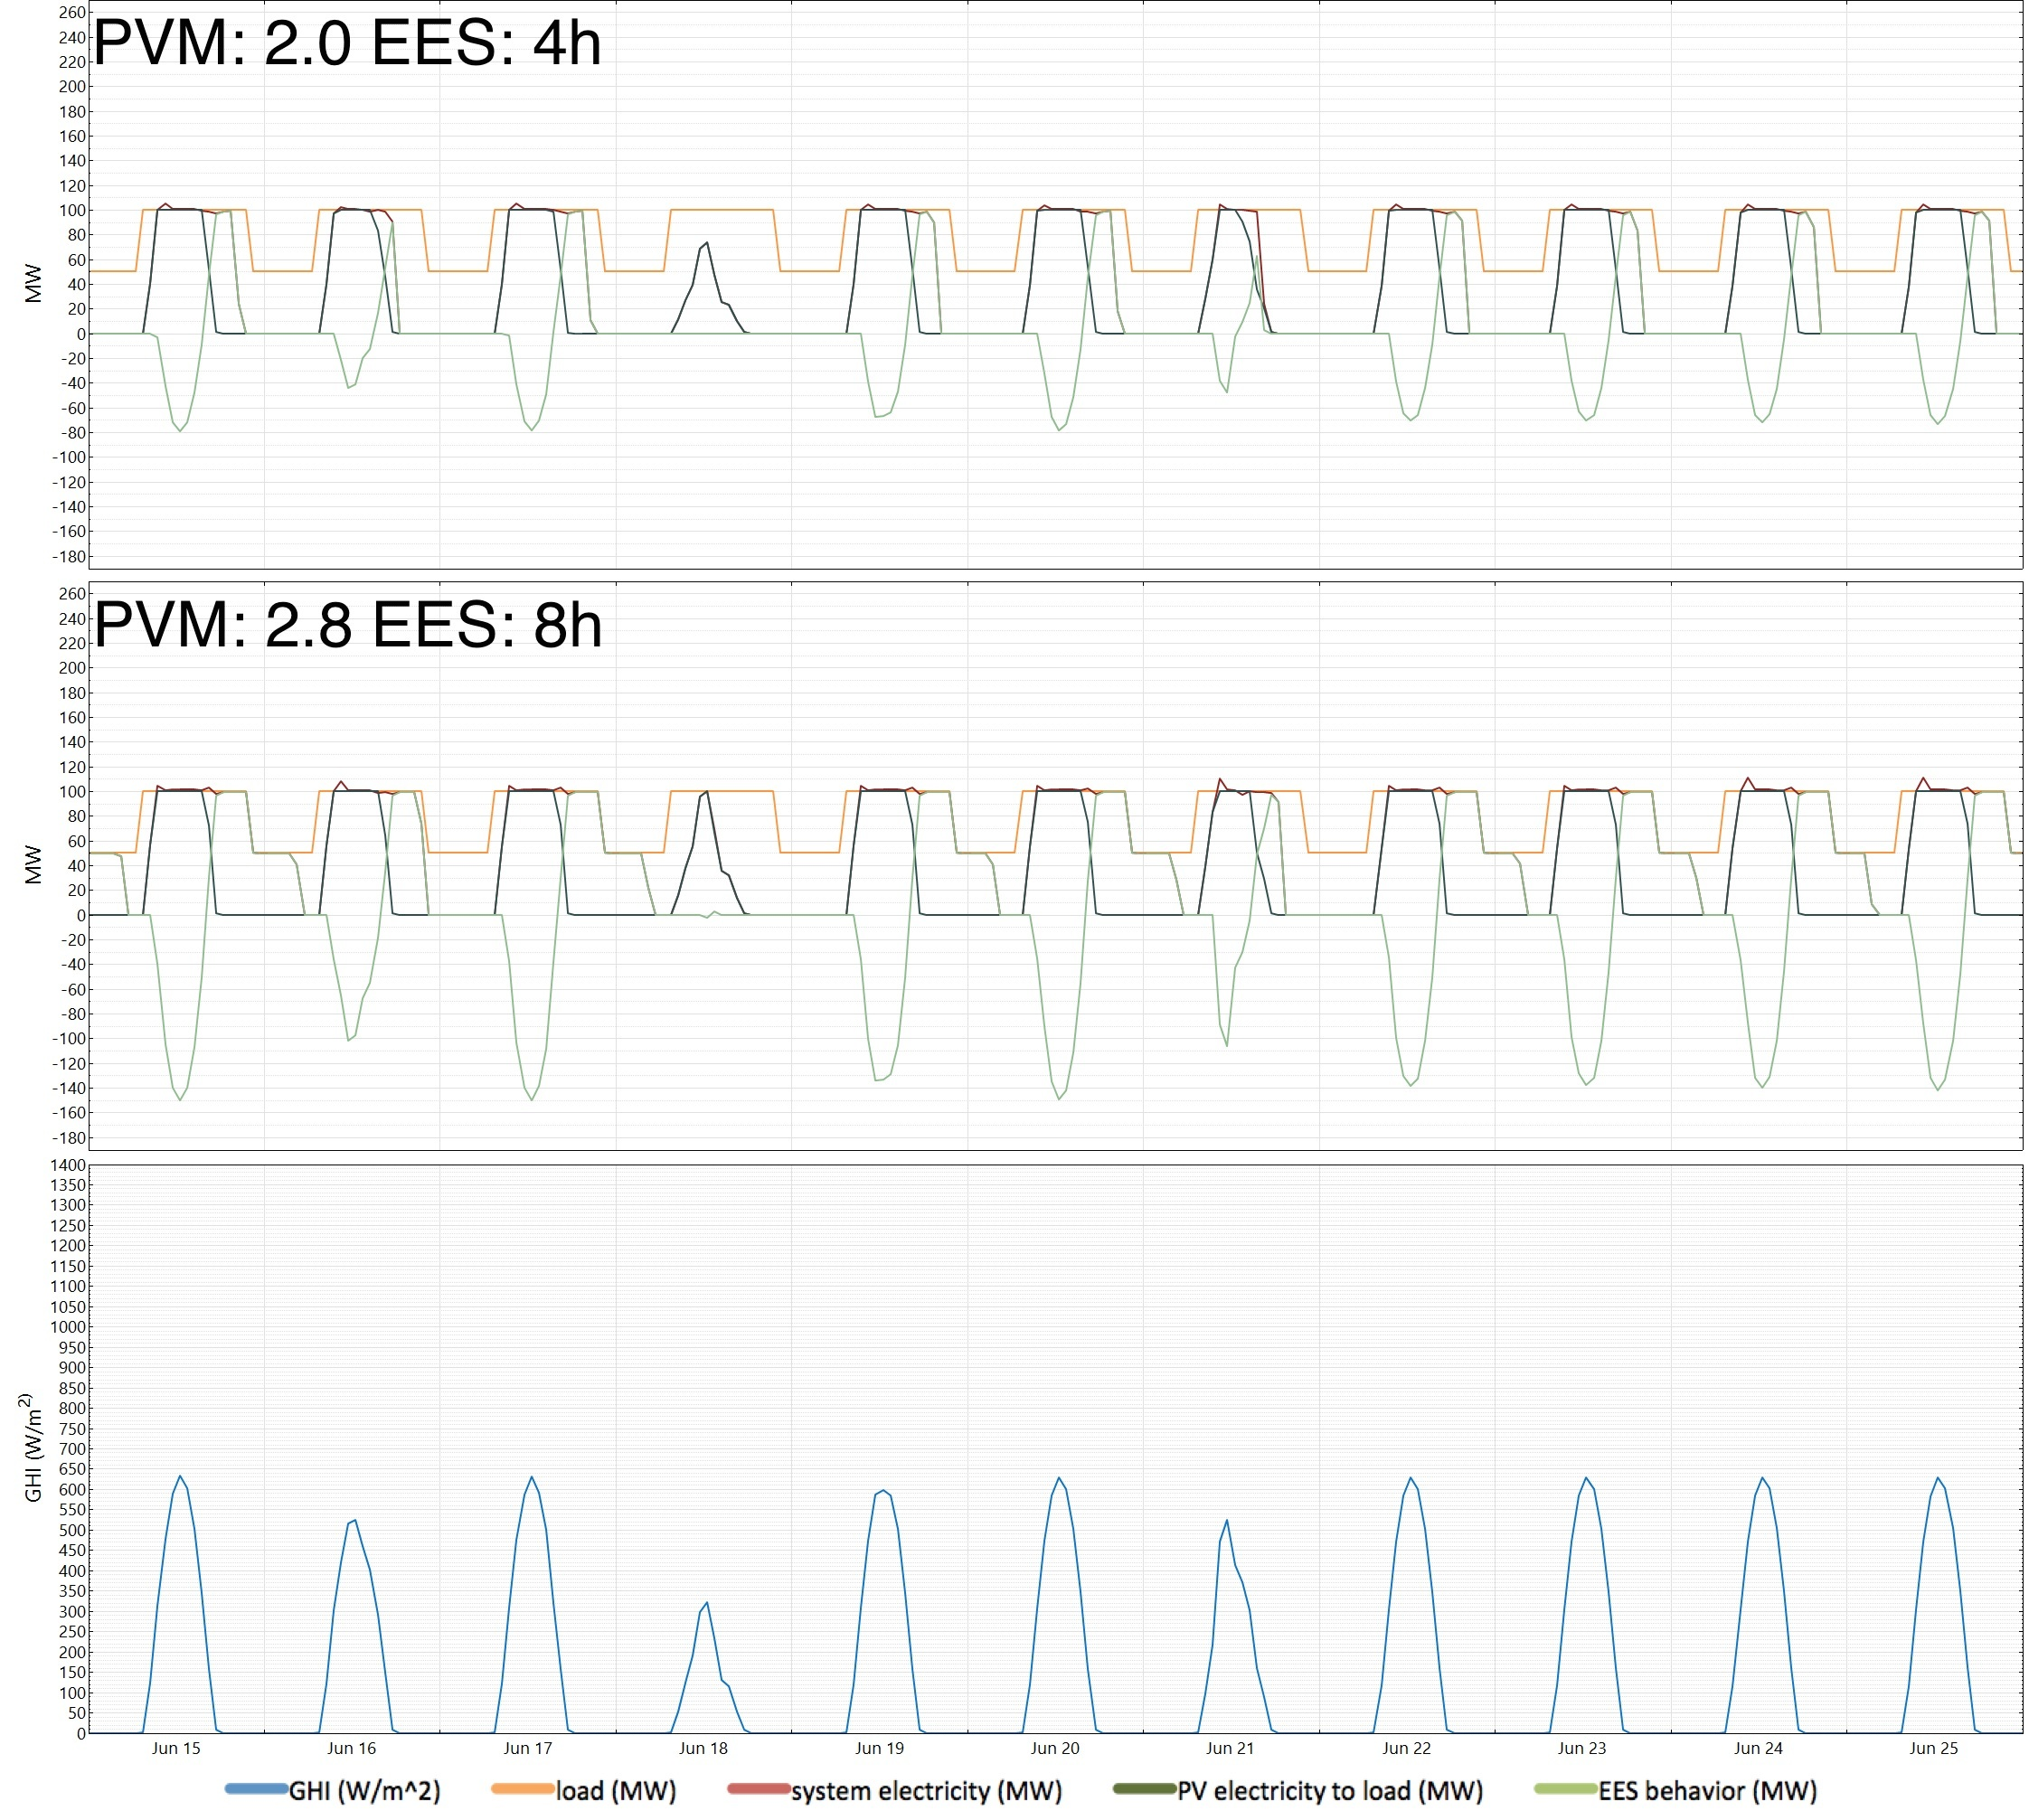
\includegraphics[width=1\linewidth]{FIG/PV_winter_load}
\caption[PV system with adapted EES load profile during the time of winter solstice.]{PV system with adapted EES load profile during the time of winter solstice (15. June - 25. June).}\label{PV_winter_load}
\end{figure}
The behavior of the power output of the selected simulated PV power plants and there power flow is shown in Figure~\ref{PV_winter_load} for the time with the lowest irradiance values. During the time of the winter solstice the value of GHI reaches just about \SI{630}{\watt\per\square\metre} in peak. The graph shows the behavior of the EES during the days and as it was described above the PV system first covers the prescribed load and then charges the EES with there surplus power. In the time span of the 22. to the 25. of June are the irradiance values of GHI during the days almost perfect. Nevertheless, both PV power plant configurations can't produce power without coming to standstill. The configuration with a PVM of 2.0 and \SI{4}{h} of EES stops covering the prescribed load before this steps down to the night reduction. But the PV power plant configuration with a PVM of 2.8 and \SI{8}{h} of EES covering the load till in the early morning hours. When comparing the value of the EES charging power it is obviously that there higher charging power peaks at a higher PVM configuration a the lower. 

During the winter times captures the EES the whole electricity power from the simulated PV systems, but this is not always the situation during the summer times. Figure~\ref{PV_summer_load} shows the load profile during the longest days of the year for the two selected configurations of the simulated PV power plants. The GHI rises up to \SI{1210}{\watt\per\square\metre} in peak at the portrayed time span.

\begin{figure}[htbp]
\centering
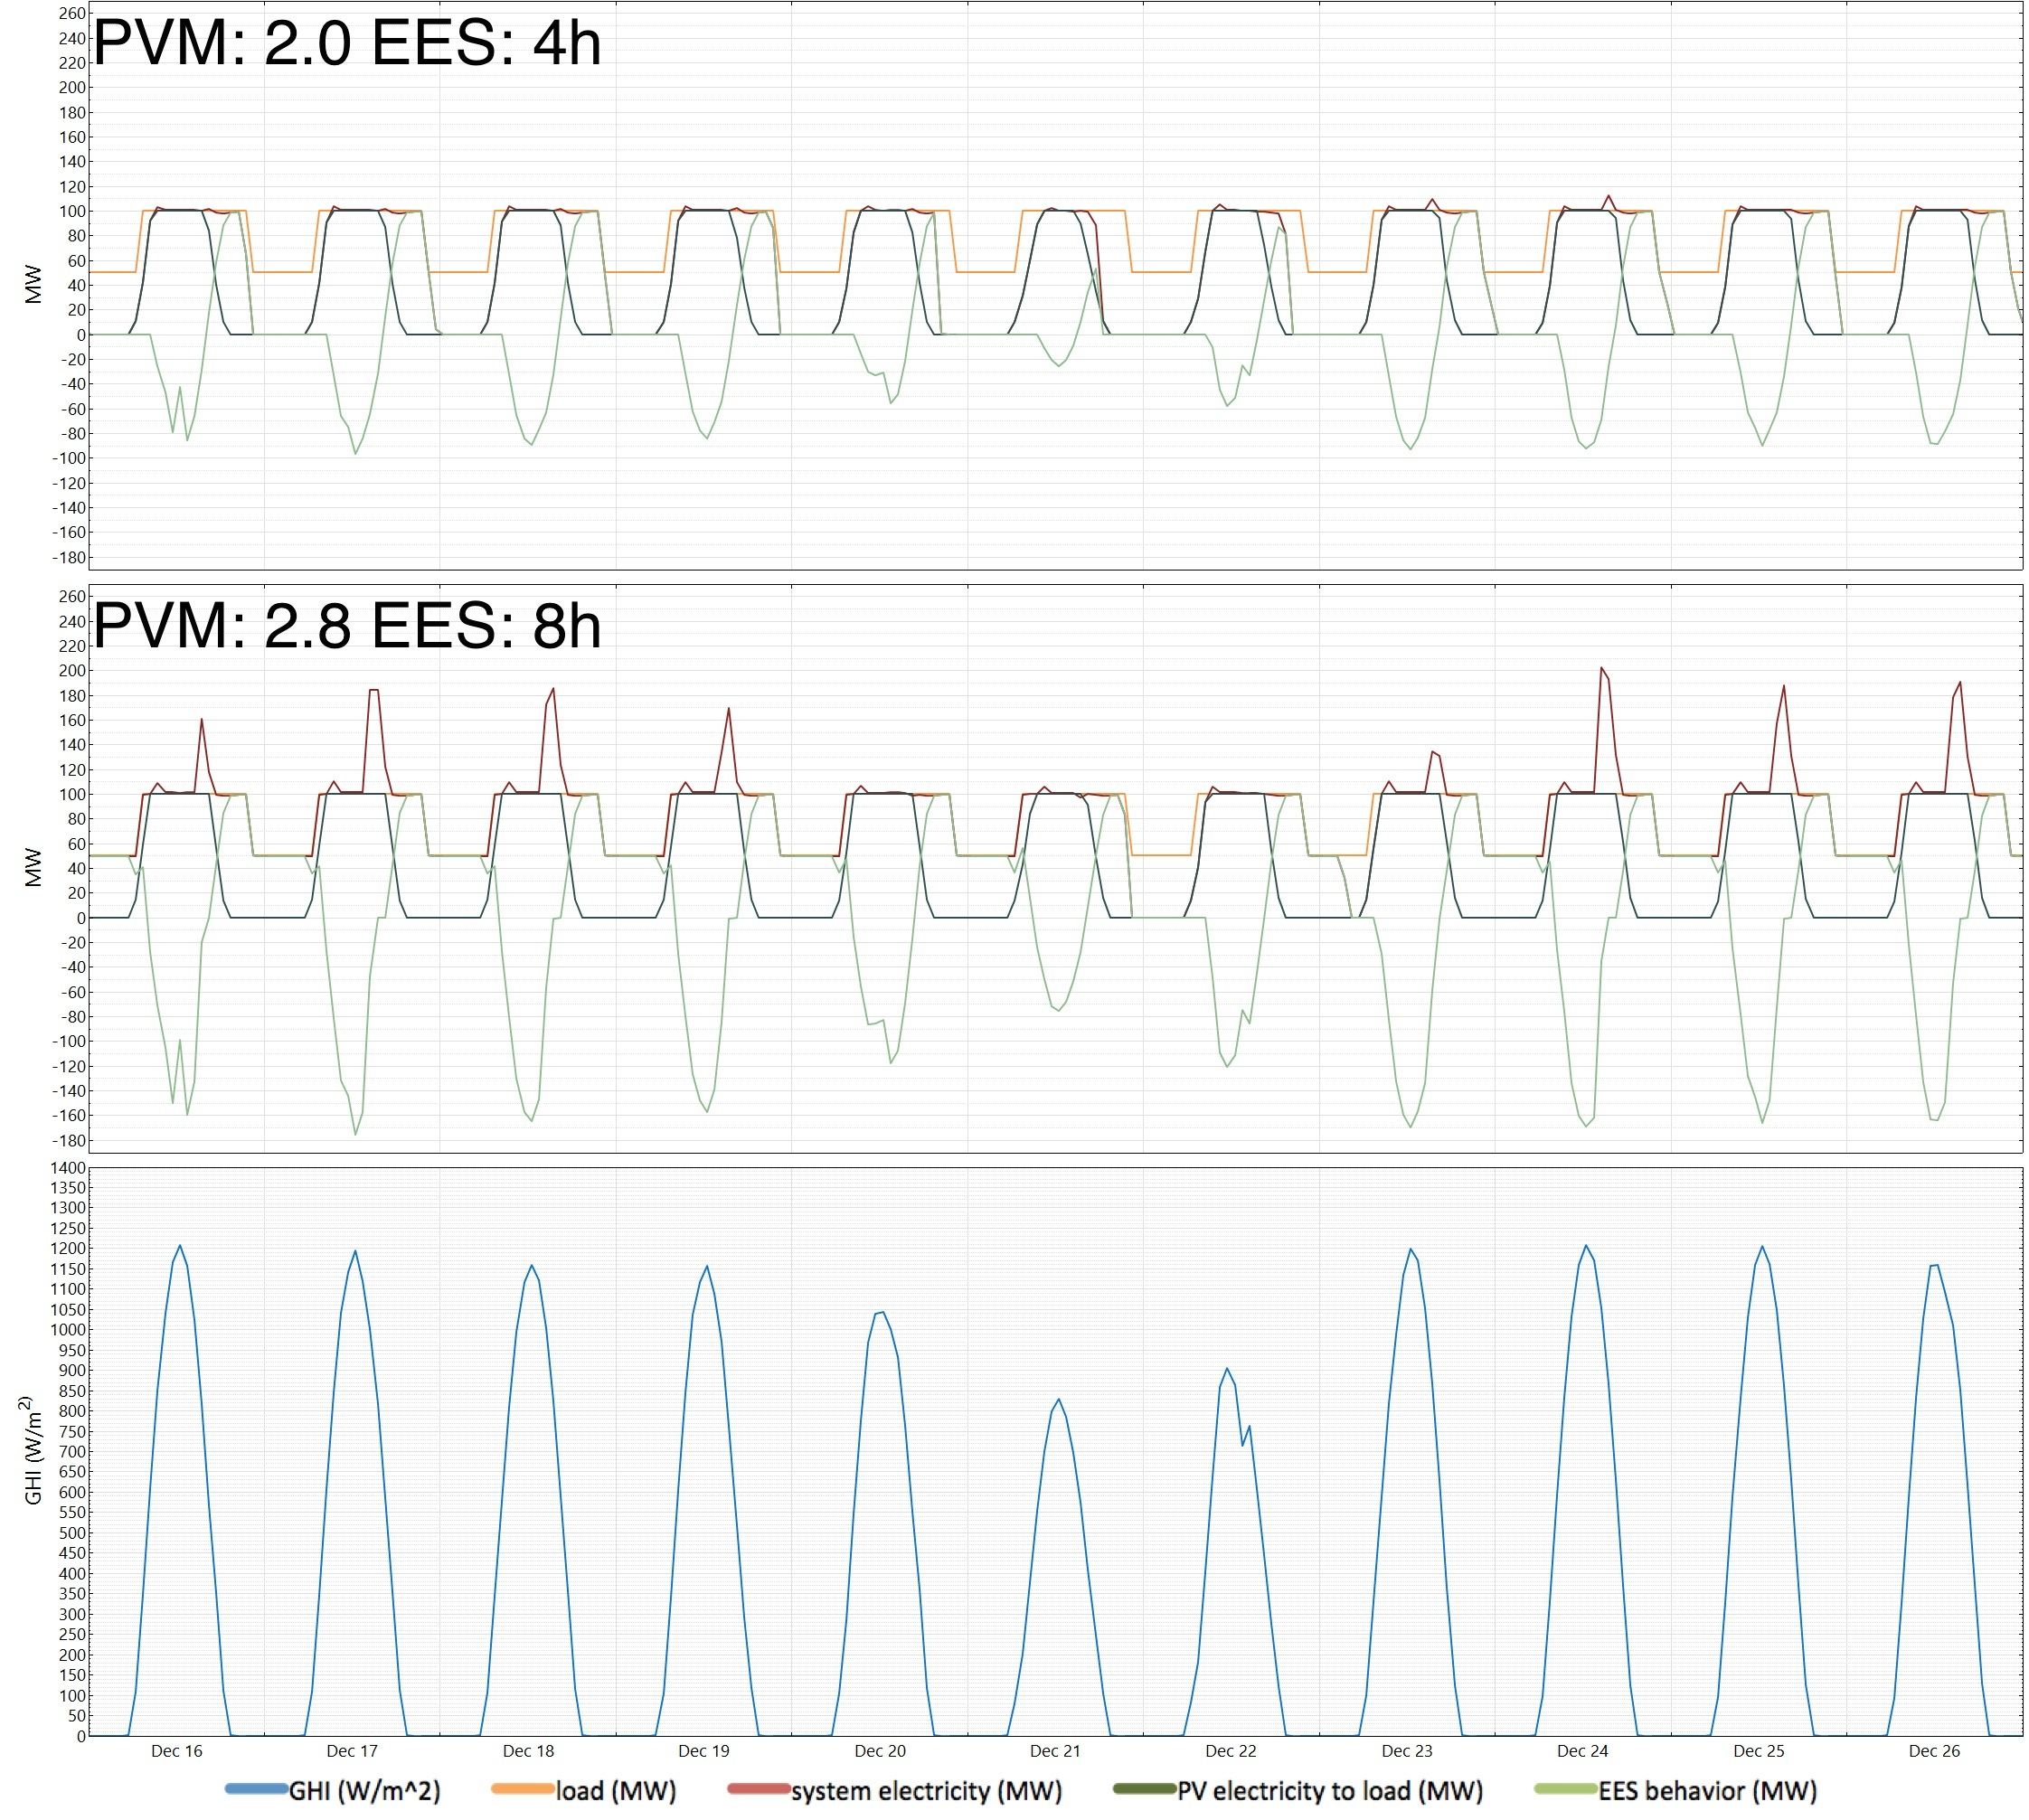
\includegraphics[width=1\linewidth]{FIG/PV_summer_load}
\caption[PV system with adapted EES load profile during the time of summer solstice.]{PV system with adapted EES load profile during the time of summer solstice (16. December - 26. December).}\label{PV_summer_load}
\end{figure}
The graph shows that the lowest PV power plant configuration can't cover the prescribed load during the night. The by the system provided power coming to stand still when the load got reduced for the night reduction at latest. Therefore the electricity production standstill during the night in the annual average load profile (Figure~\ref{PV_annual_profil}) as well. In comparison to that covers the highest PV power plant configuration almost the full prescribed load. Just during the following night times of days with lower irradiance (21. \& 22. December) comes the systems electricity output to standstill. Considering the system electricity output more precise, it offers high overproduction peaks which are the above mentioned situations where the storage got full charged and the PV system produces more power than the load requests.  

This surplus output depends on the ratio between the PV and EES system. The behavior of the ratio is shown in Figure~\ref{PV_energy_output}, which describes the share of the PV power plants energy output in the first year. The chart shows that the share of surplus energy rises with a higher PVM and decreases by larger EES capacity.

\begin{figure}[htbp]  
\centering
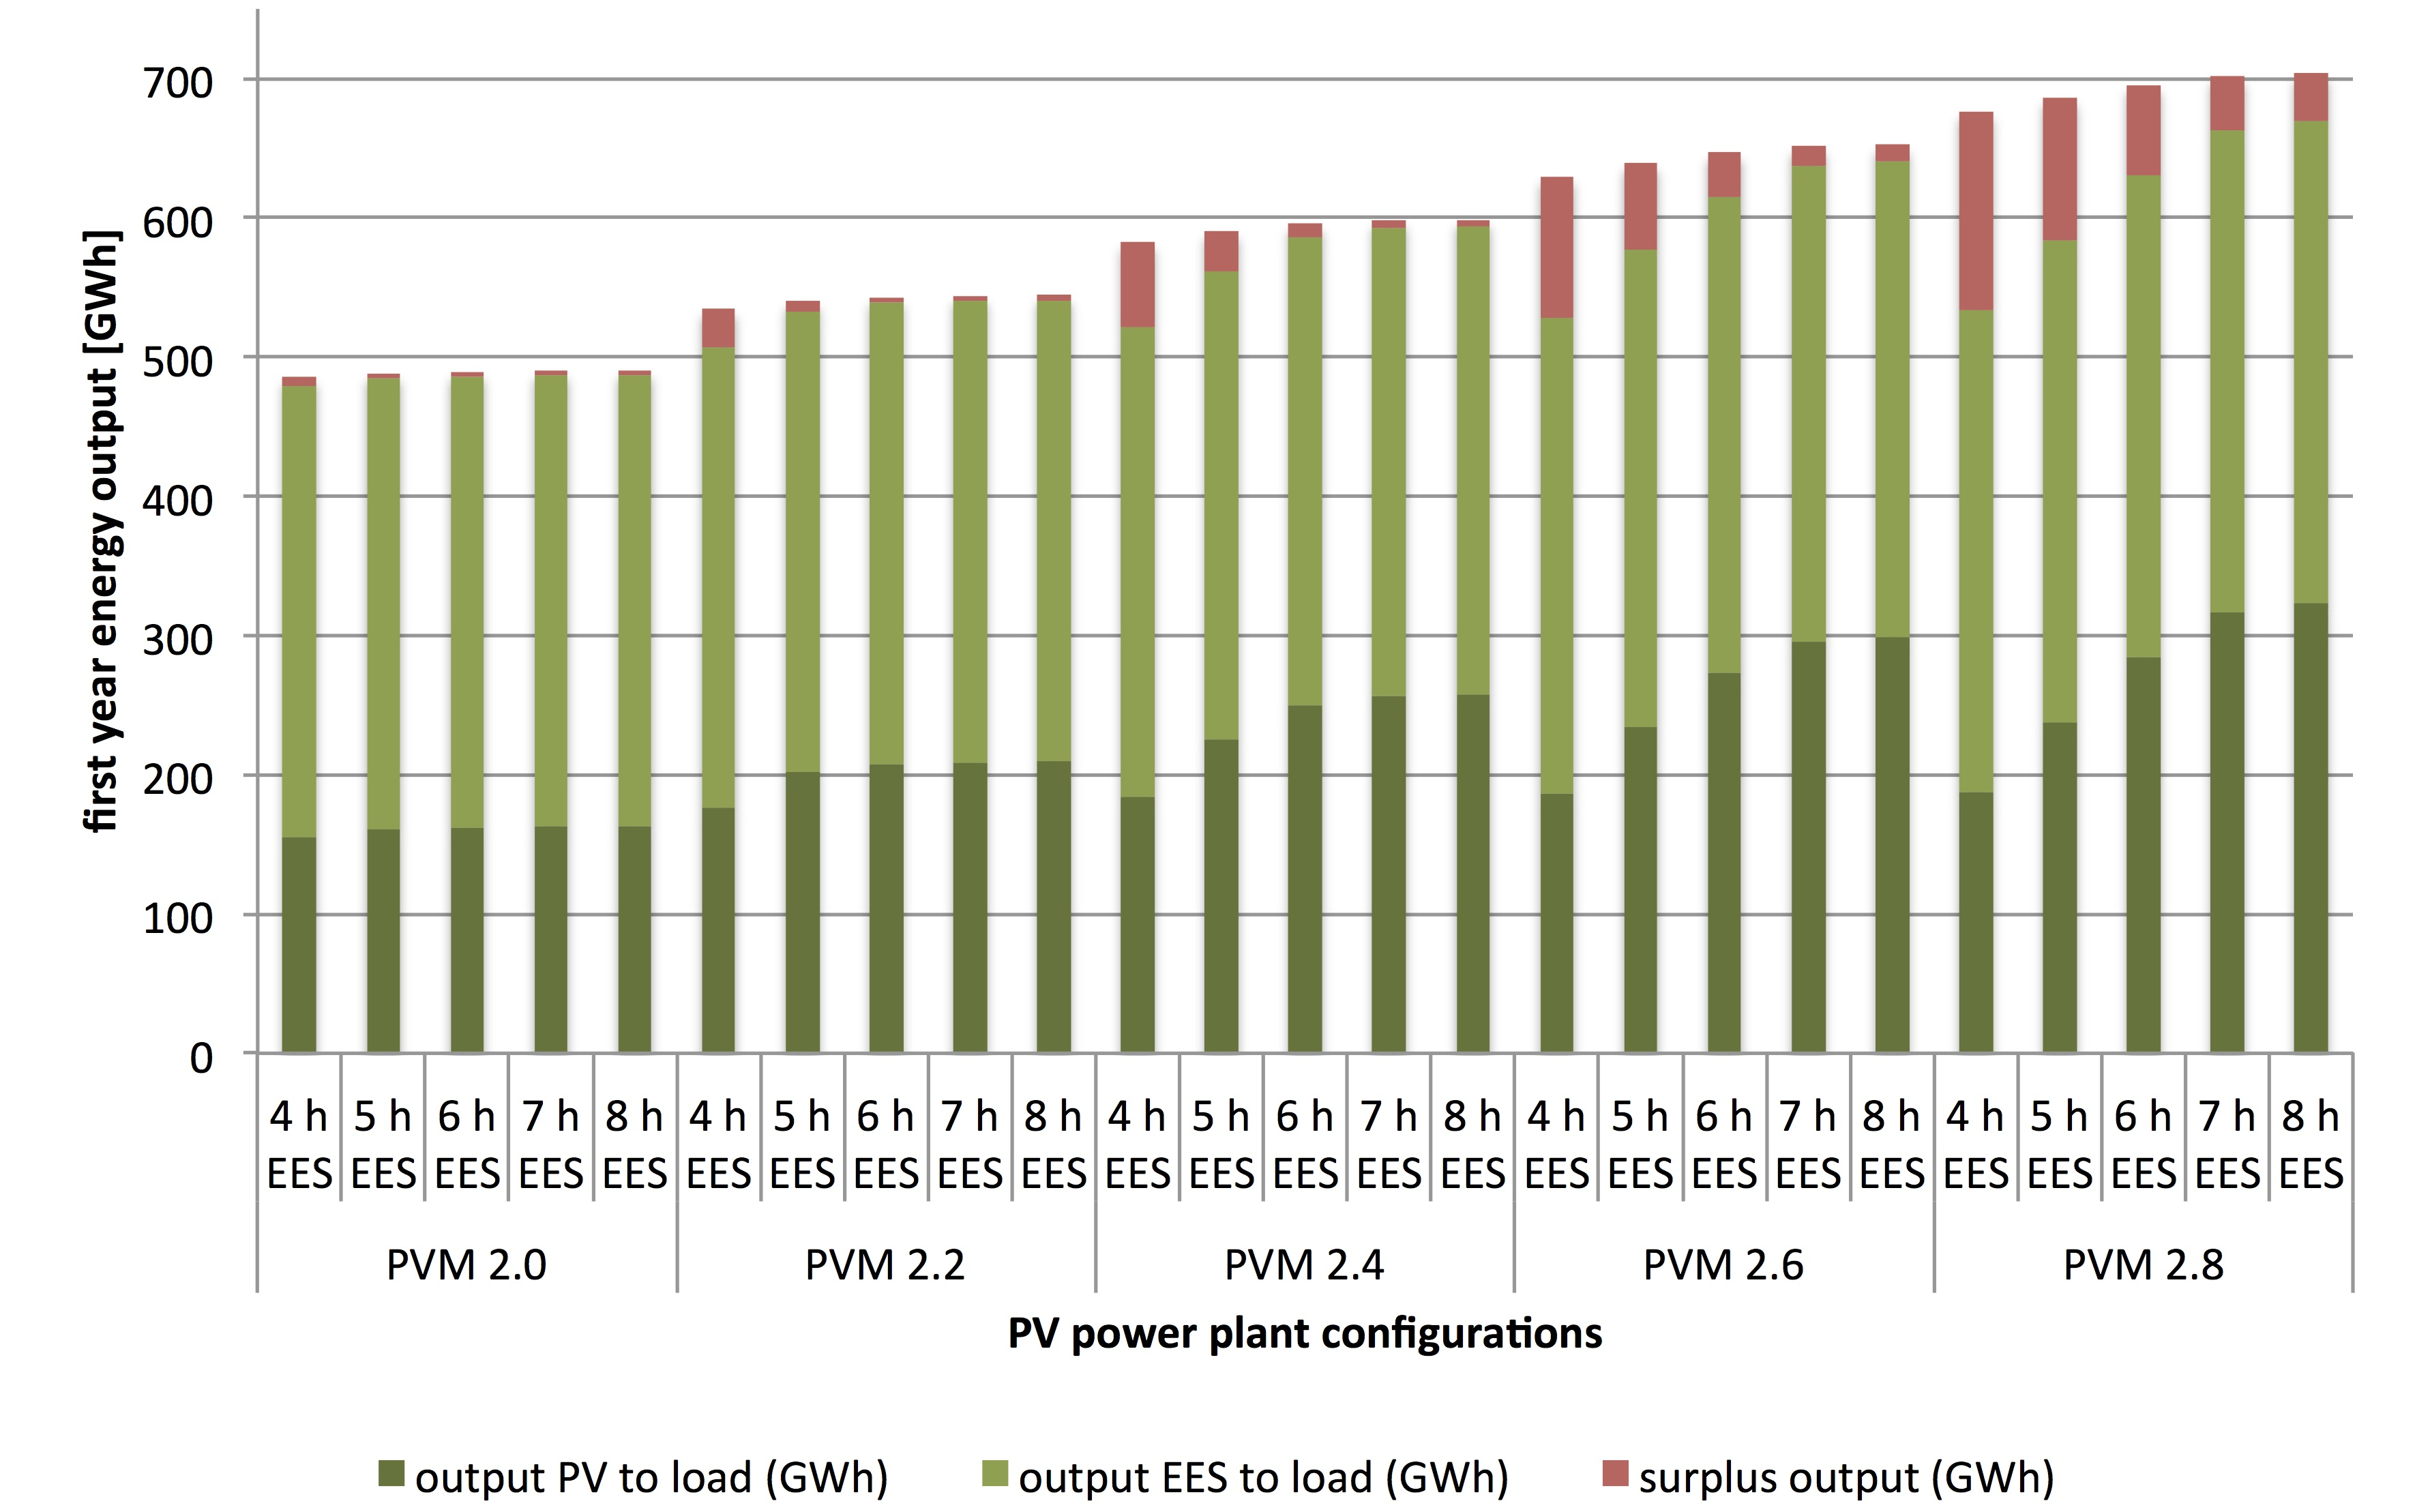
\includegraphics[width=1\linewidth]{FIG/PV_energy_output}
\caption[Share of energy output of all simulated PV power plants with adapted EES.]{Share of energy output of all simulated PV power plants with adapted EES.}\label{PV_energy_output}
\end{figure}
The Figure also gives an idea of the amount of the energy output of the simulated PV power plants for covering the prescribed load. The lowest simulated configuration produces an energy output of about \SI{479.54}{GWh} in the first year which covers the prescribed load. The total sum of the annual prescribed load is \SI{711.75}{GWh}. Consequently, the lowest configuration of the simulated PV power plants covers 67.4~\% of the prescribed load in the first year. The share of the surplus output is 1.2~\% of the total generated energy. The energy output of the highest simulated configuration has a share of a surplus output of about 4.9~\% and produces an load covering energy output of about \SI{669.44}{GWh} in the first year. This output covers 94.1~\% of the prescribed load.

The from the energy output derived load curve covering results of the simulated PV power plant are shown in Figure~\ref{PV_LCCF}. At a PVM of 2.0 the size of the variations of EES don't have a big influence to the load curve covering. With the rising PVM the significance of the EES capacity gains as well. The forced target to covering 90~\% of the prescribed load is reached with the EES configuration 7 and \SI{8}{h} from a PVM of 2.6 on. The configuration PVM 2.6 with \SI{7}{h} of EES reaches actually just about 89.58~\% but reaching the 90~\% by round up. 70~\% load covering is reached by all EEs capacities and besides of the \SI{4}{h} EES configuration also all simulated EES variants reaching the covering of 80~\% of the prescribed load. 

\begin{figure}[htbp]  
\centering
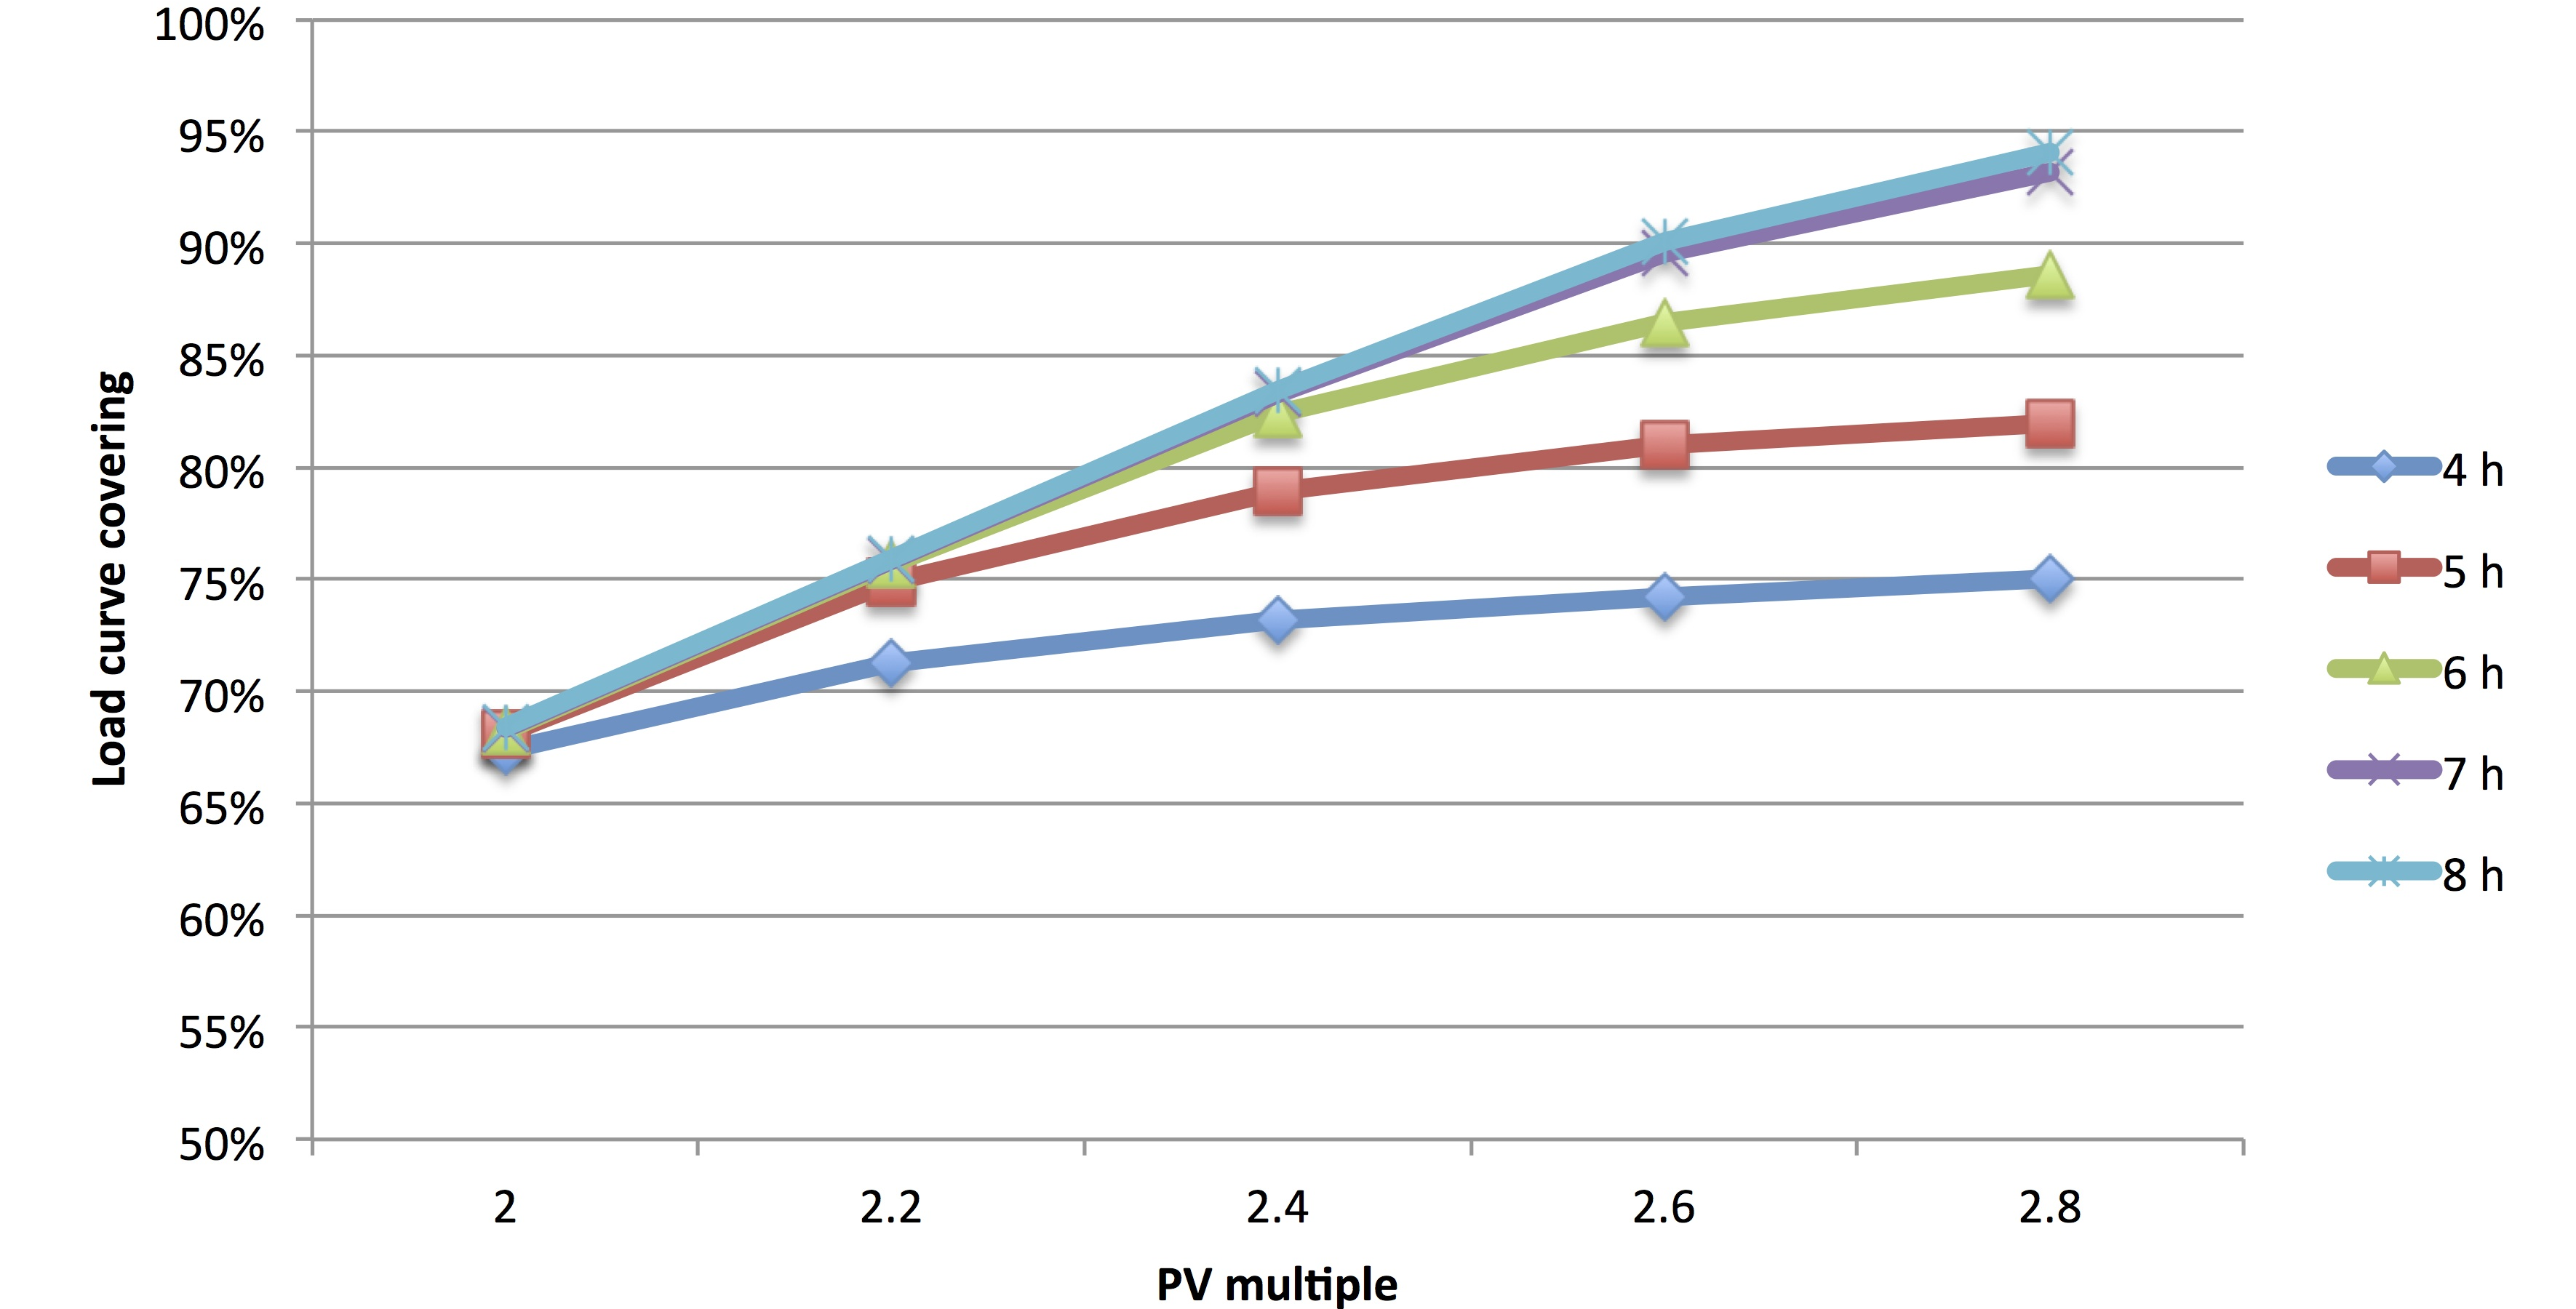
\includegraphics[width=1\linewidth]{FIG/PV_LCCF}
\caption[Load curve covering result of simulated PV systems with adapted EES.]{Load curve covering result of simulated PV systems with adapted EES.}\label{PV_LCCF}
\end{figure}
\pagebreak
\subsubsection{Levelized costs of electricity}
The LCOE was calculated by using the finacial input parameter from Table~\ref{tbl: PVFinance} and a simplified method which is documented in Appendix~\ref{ChapterLCOE} on Page \pageref{ChapterLCOE}. It must be noted, that the calculation is based on the simulation result for the first year PV power plant results under consulting of a degradation factor for the PV system, but not for the EES. The results of the LCOE claculation for the simulated PV power plant configurations can be seen in Figure~\ref{PV_LCOE}. 

The lowest LCOE result of \SI{251.83}{USD/MWh} is reached at a PVM of 2.2 and the lowest EES configuration and is marginal lower than  \SI{252.42}{USD/MWh} at a PVM of 2.4 with the same EES configuration. Generally must be said that there are no overlaps of LCOE lines in this chart and the spacing leads from the EES system costs.

\begin{figure}[htbp]  
\centering
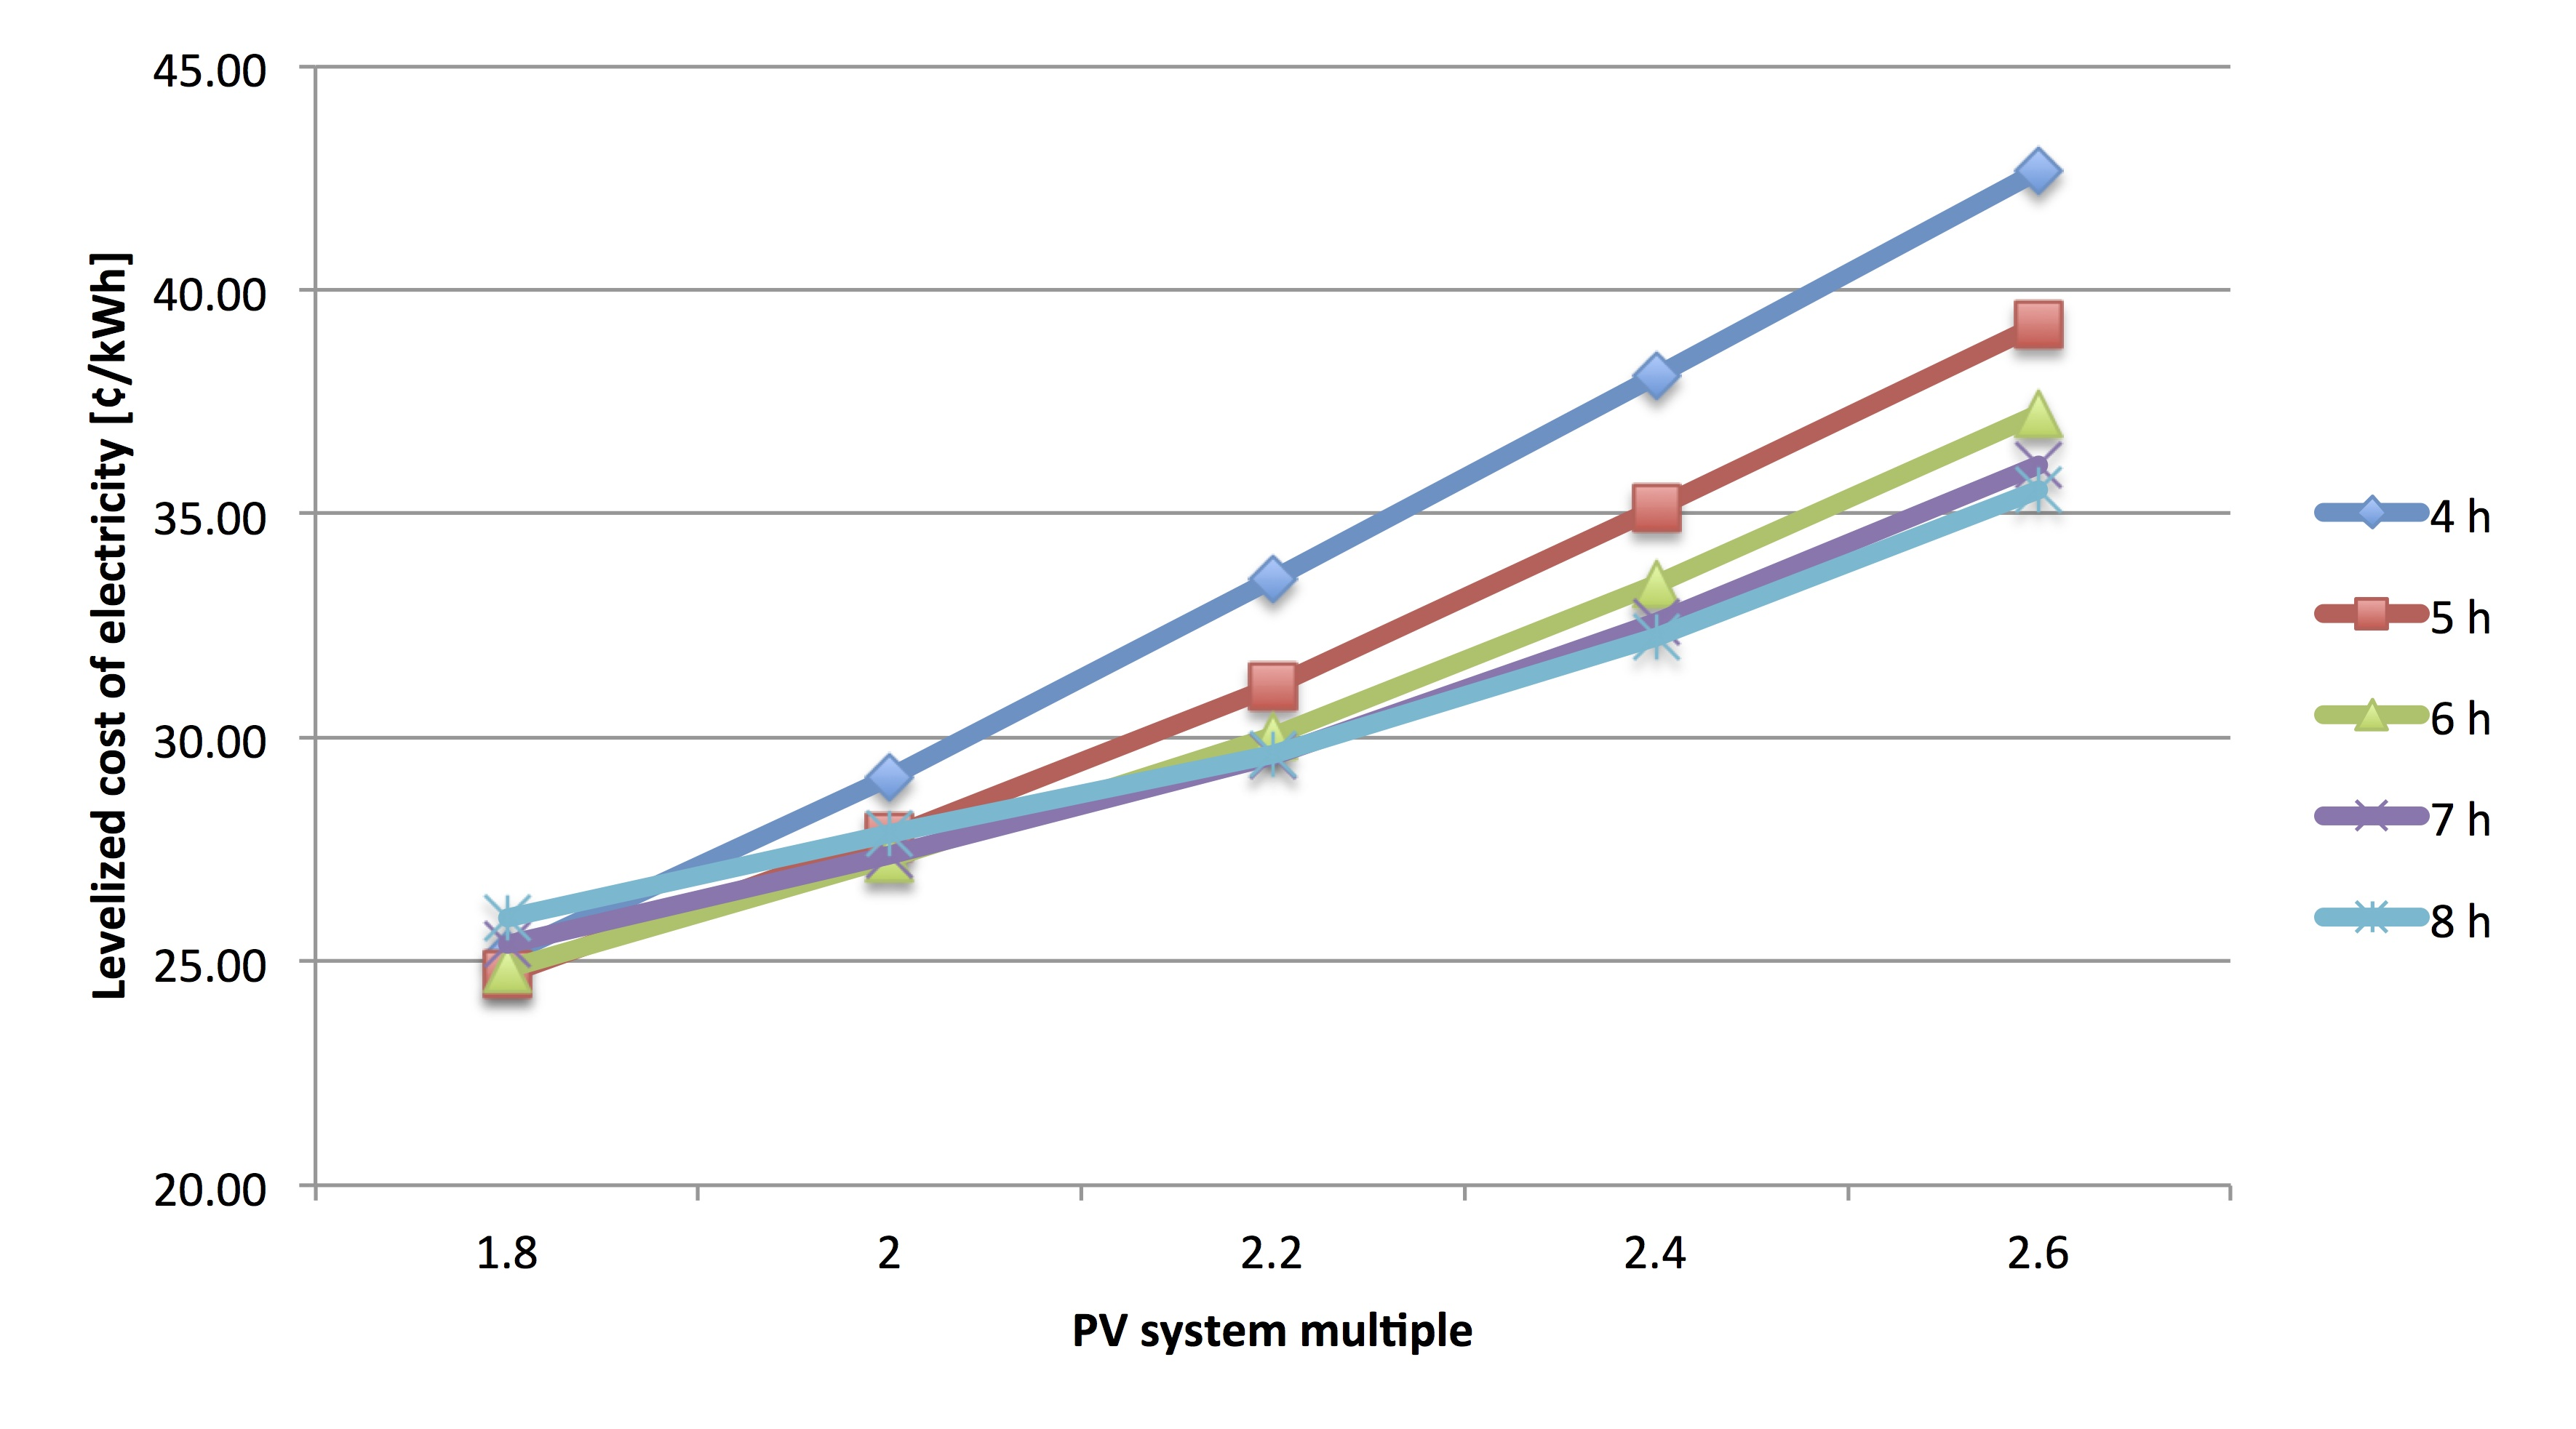
\includegraphics[width=1\linewidth]{FIG/PV_LCOE}
\caption[LCOE calculation results for PV systems with adapted EES simulation.]{LCOE calculation results for PV systems with adapted EES simulation.}\label{PV_LCOE}
\end{figure}
The EES systems costs share makes the main part of the LCOE cost of the simulated PV power plants with an adapted EES. The break-down of the LCOE is shown for the lowest and highest configuration in Figure~\ref{SMPV_LCOE_BreakDown}. This chart clarify the big impact of the EES cost. At the lowest configuration 81~\% of the LCOE are traced to the EES and at the highest about 86~\%. The other results showed that the range of the EES is between 76\% and 89~\% of the calculated LCOE's.

\begin{figure}[!htbp]
        \centering                
        \begin{subfigure}[b]{0.5\textwidth}
                \centering
                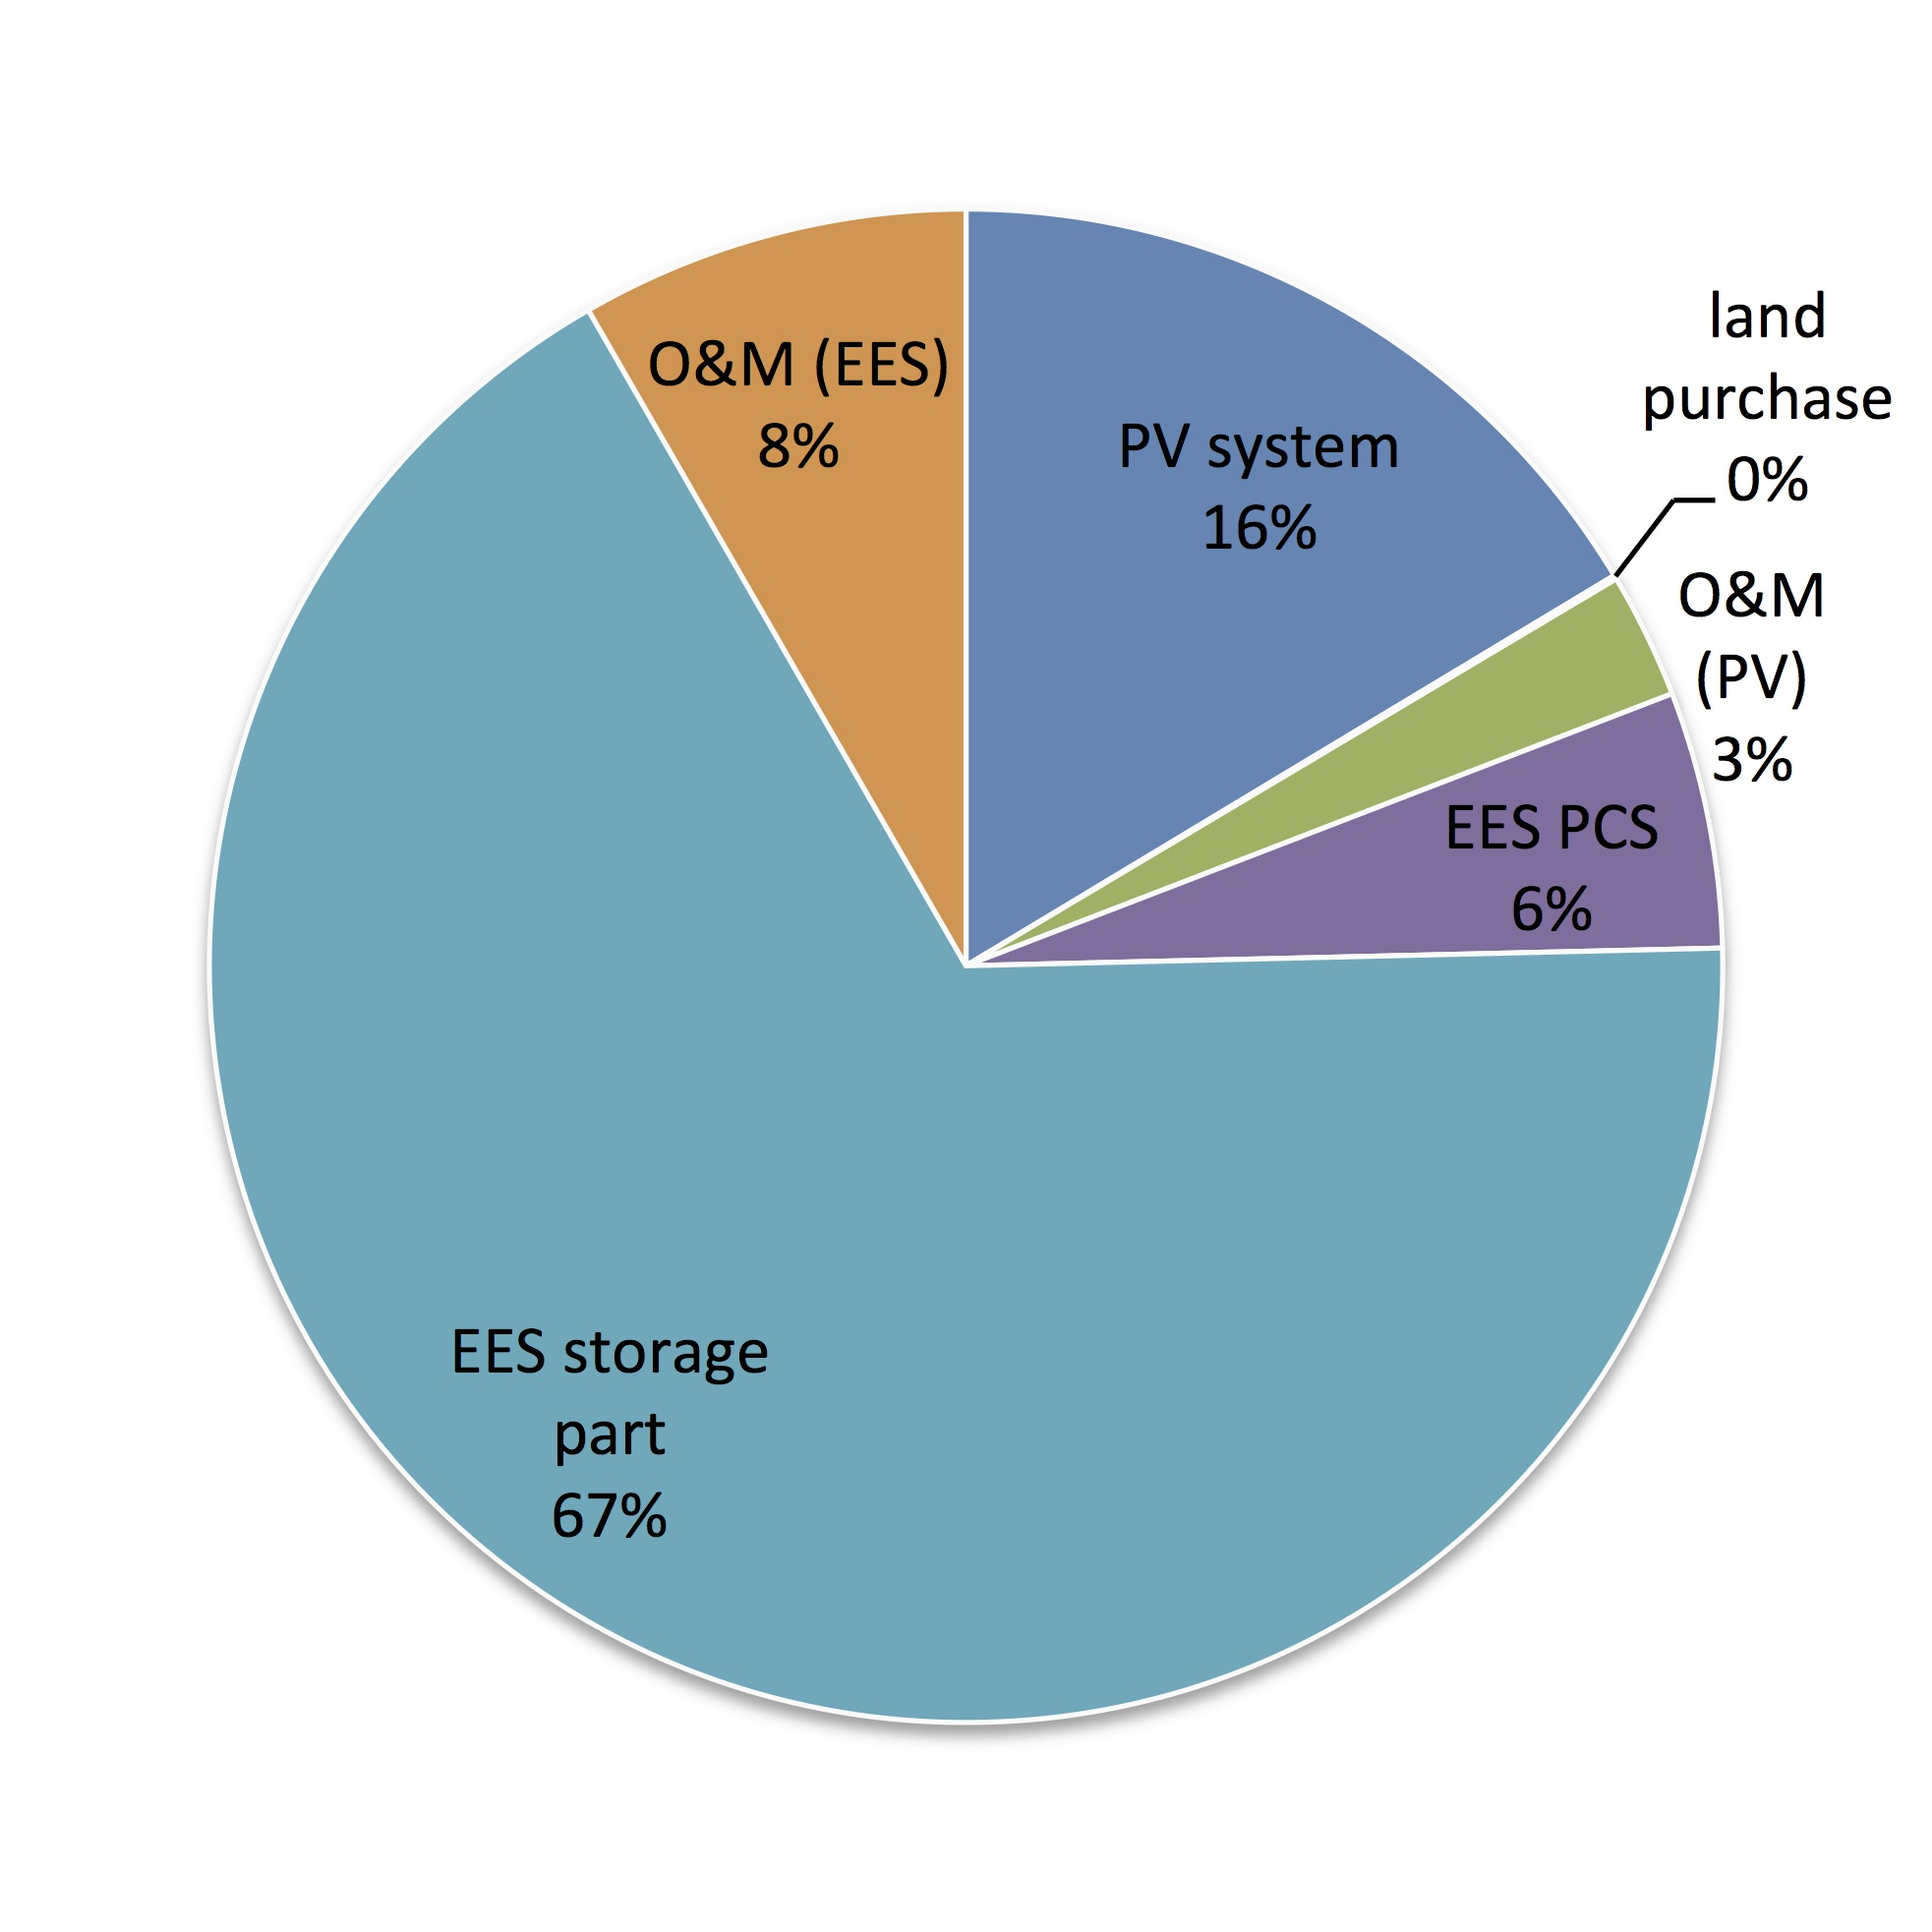
\includegraphics[width=1\textwidth]{FIG/PV_LCOE_lowinvest_BreakDown}
                \caption{LCOE break-down for PVM~2.0 and \SI{4}{h}~EES.}\label{PV_LCOE_lowinvest_BreakDown}
        \end{subfigure}%
        ~
        \begin{subfigure}[b]{0.5\textwidth}
                \centering
                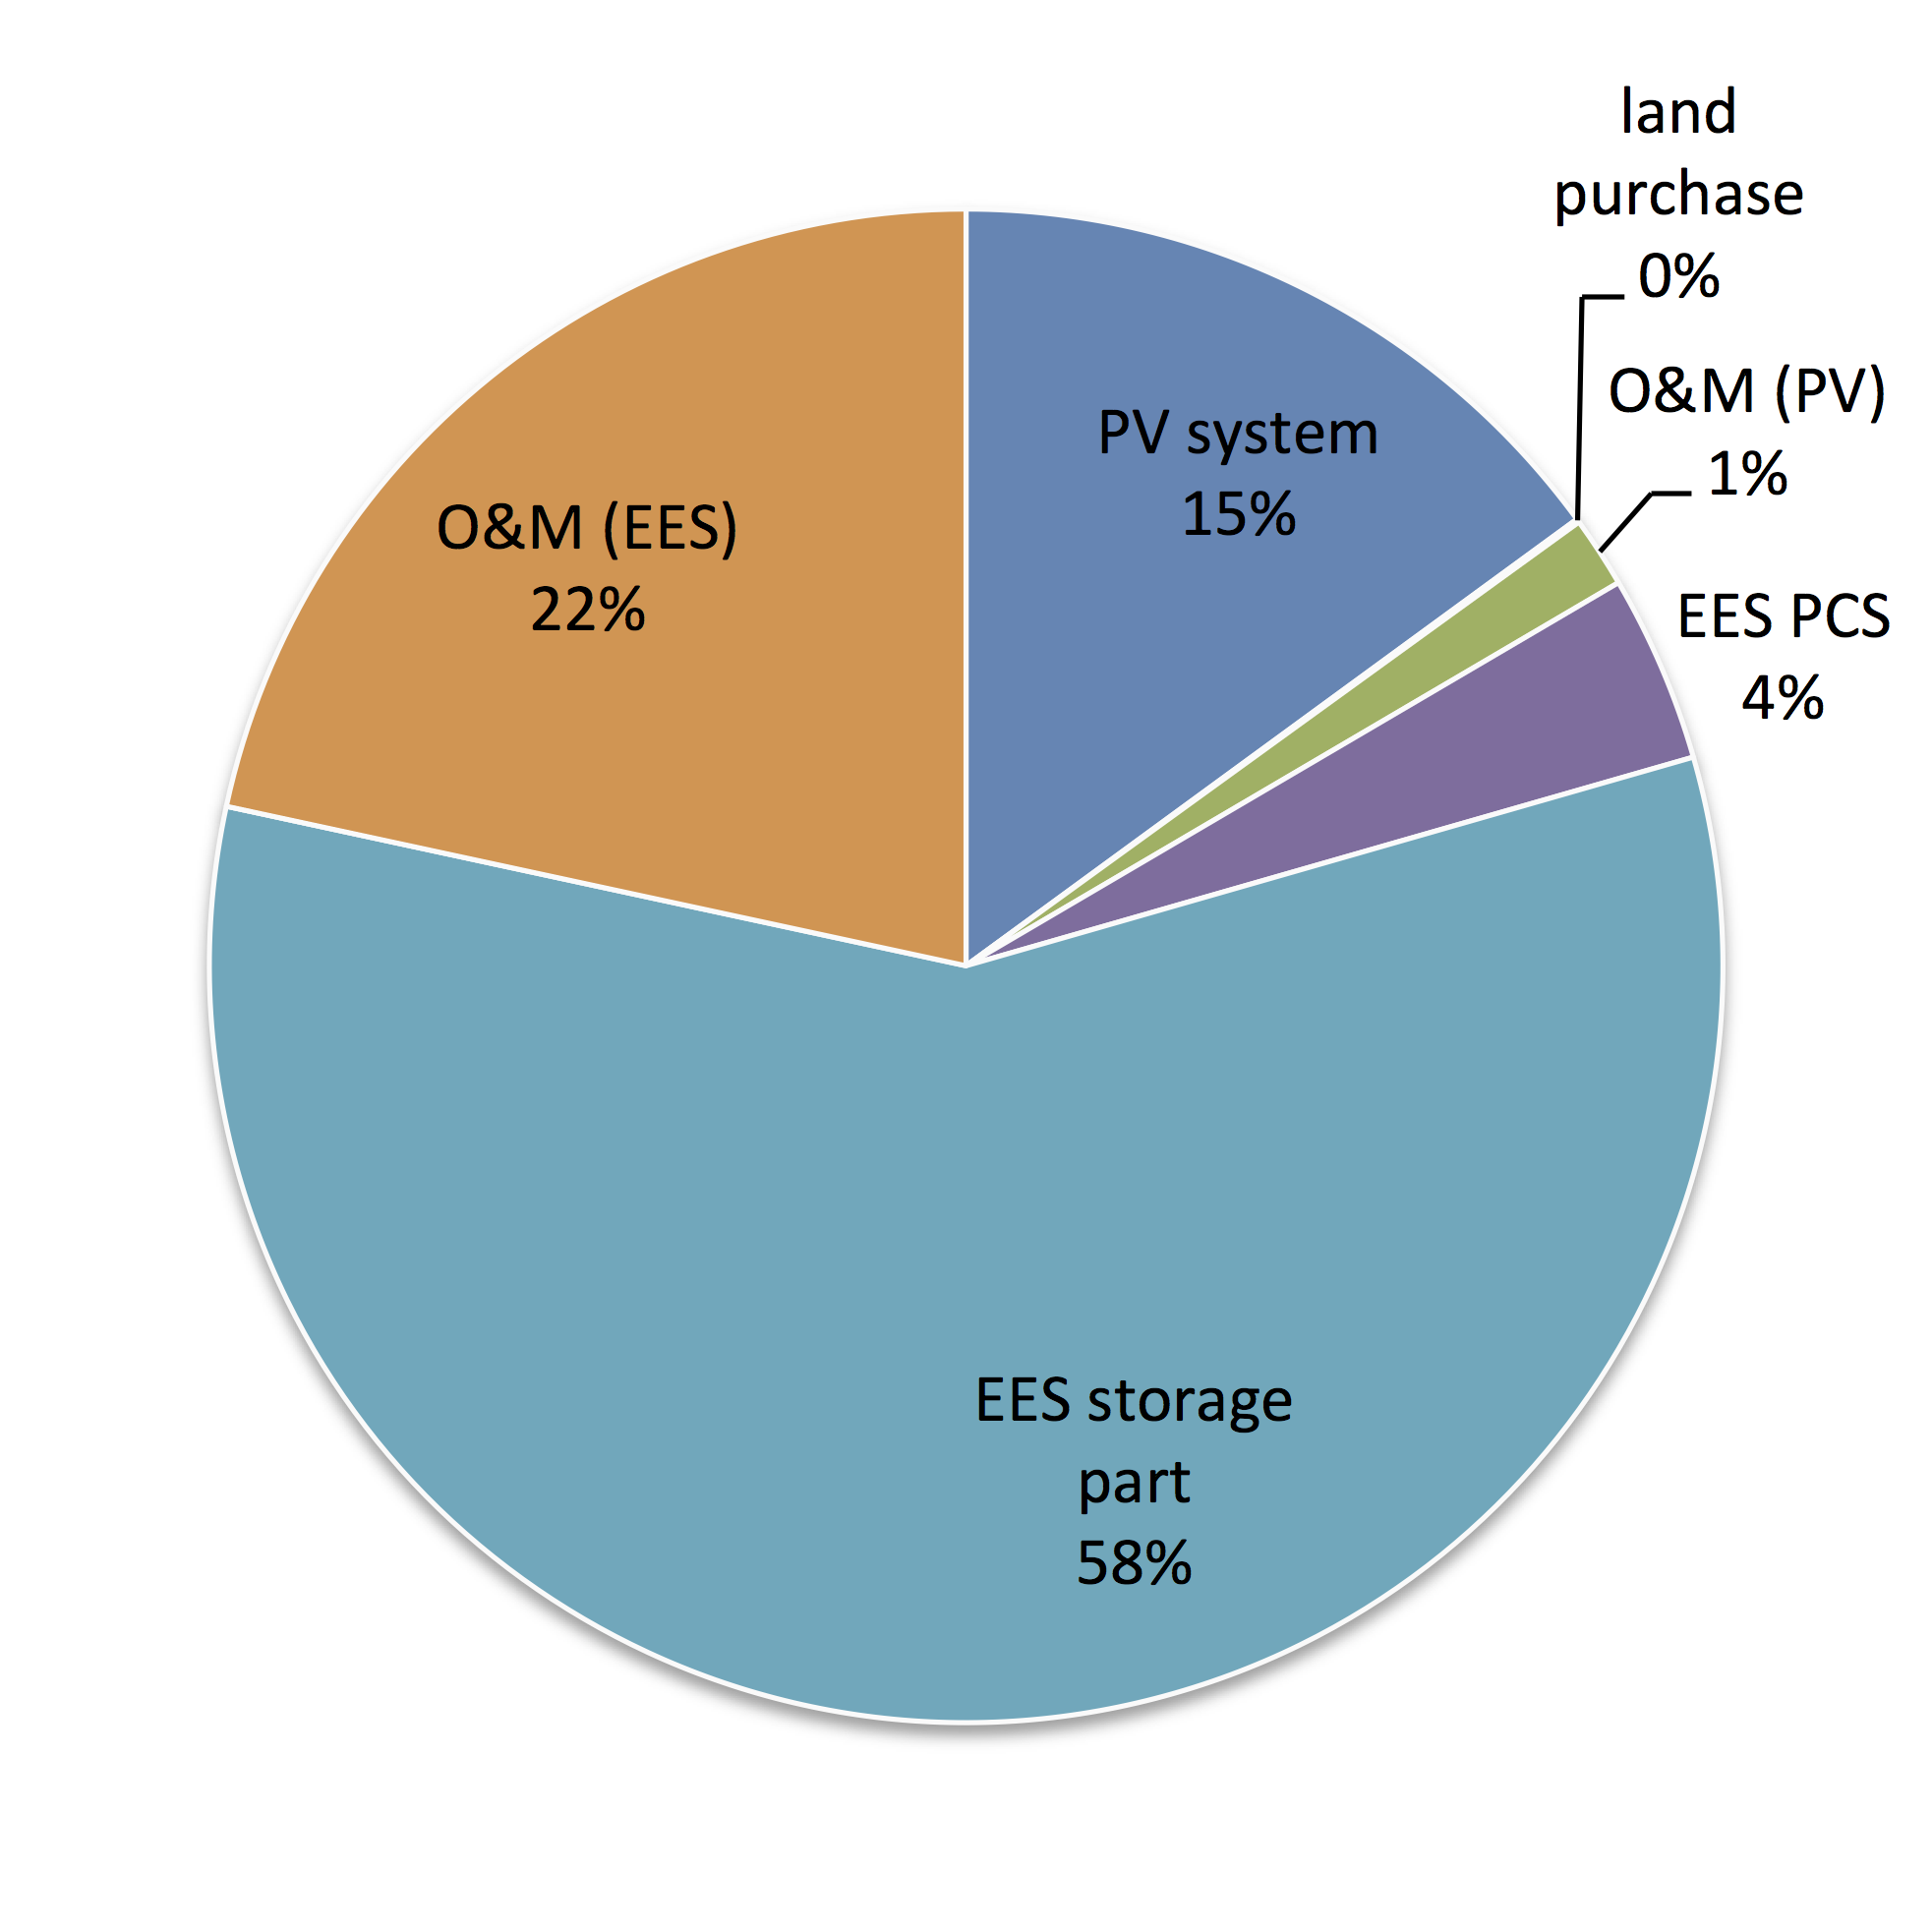
\includegraphics[width=1\textwidth]{FIG/PV_LCOE_highinvest_BreakDown}
                \caption{LCOE break-down for PVM~2.8 and \SI{8}{h}~EES.}\label{PV_LCOE_highinvest_BreakDown}
        \end{subfigure}
        \caption[Break-down of selected LCOE calculation  results of PV systems with adapted EES.]{Break-down of selected LCOE calculation results of PV systems with adapted EES.}\label{SMPV_LCOE_BreakDown}
\end{figure}
Comprising the results of the LCOE calculation and associated load curve covering results shows that for covering 90\% of the predicted load the configuration of PVM 2.8 and \SI{7}{h} of EES reaching the lowest LCOE of \SI{315.39}{USD/MWh}. But the configuration owns an high value of surplus output of about 5.5~\% (see Figure~\ref{PV_energy_output}). The configuration PVM 2.6 reaches also the 90~\% load curve covering with a share of just 2.1~\% surplus output and a LCOE of \SI{322.18}{USD/MWh}.

The lowest LCOE for reaching 80~\% of the prescribed load is \SI{275.18}{USD/MWh} using \SI{5}{h} of EES and also a PVM of 2.6. For reaching 70~\% the 2.2 and \SI{4}{h} of EES reaches the lowest LCOE of \SI{251.83}{USD/MWh}.
\pagebreak